\documentclass[12pt]{article}
\usepackage[utf8]{inputenc}
\usepackage{geometry}
\geometry{a4paper, margin=1in}
\usepackage{graphicx}
\usepackage{tabularx}
\usepackage{longtable}
\usepackage{hyperref}
\usepackage{listings}
\usepackage{placeins}

\title{Verification and Validation Report: Angry Bird Alike}
\LARGE\author{Author: Hossain, Al Jubair}
\date{April 3, 2024}

\begin{document}

\maketitle

\newpage
\tableofcontents
\listoftables
\listoffigures
\newpage

\section*{Revision History}
\begin{longtable}{|p{2cm}|p{2cm}|p{10cm}|}
    \hline
    \textbf{Date} & \textbf{Version} & \textbf{Notes} \\
    \hline
    April 3, 2024 & 1.0 & Initial Version.\\\hline
    April 3, 2024 & 1.5 & Revised based on feedback and changes from SRS, VnV Plan, MG and MIS.\\
    \hline
\end{longtable}
\addcontentsline{toc}{section}{Revision History}
\FloatBarrier

\newpage
\section*{Symbols, Abbreviations and Acronyms}
\begin{tabular}{|l|l|}
\hline
Symbol & Description \\
\hline
T & Test \\
\hline
P & Pass\\
\hline
F & Fail\\
\hline
FR & Functional Requirement \\
\hline
NFR & Non-Functional Requirement \\
\hline
UI & User Interface \\
\hline\hline
\end{tabular}
\addcontentsline{toc}{section}{Symbols, Abbreviations and Acronyms}
\FloatBarrier

\section{Functional Requirements Evaluation}

Our functional requirements were comprehensively tested through unit testing using the Catch2 framework. Here, we summarize the evaluation of several key functionalities:

\subsection{Degrees to Radians Conversion}
\textbf{Test Case:} Verify that angle conversion from degrees to radians is accurate. \\
\textbf{Outcome:} Passed. The function accurately converts angles, with tests confirming that 180 degrees equals approximately 3.14159 radians, and 90 degrees equals approximately 1.5708 radians.

\subsection{Apply Force Changes Velocity}
\textbf{Test Case:} Validate that applying force to entities correctly changes their velocity. \\
\textbf{Outcome:} Passed. Applying a force of 100.0 at a 45-degree angle correctly resulted in X and Y velocity components of approximately 70.71, adhering to the expected physical model.

\subsection{Collision Detection}
\textbf{Test Case:} Ensure accurate collision detection between entities. \\
\textbf{Outcome:} Passed. Entities positioned within collision range were correctly detected as colliding, whereas repositioning an entity out of range ceased collision detection.

\subsection{Game Reset Mechanism}
\textbf{Test Case:} Confirm that the game can be reset to its initial state. \\
\textbf{Outcome:} Passed. After applying an initial force and then resetting, the projectile's state was successfully returned to initial conditions, indicating a functional reset mechanism.

\subsection{Projectile Launch at Various Angles}
\textbf{Test Case:} Test projectile velocity at 0, 45, and 90-degree angles. \\
\textbf{Outcome:} Passed. The projectile's velocity components matched expected values for each angle, demonstrating accurate force application and motion simulation.

\subsection{Entity Immobility After Collision}
\textbf{Test Case:} Verify entities become immobile after collision. \\
\textbf{Outcome:} Passed. Upon simulating a collision, entities were correctly set to an immobile state, indicating proper collision handling.

\subsection{Entity Gravity Effect}
\textbf{Test Case:} Check the effect of gravity on projectile velocity. \\
\textbf{Outcome:} Passed. A vertically launched projectile experienced a decrease in Y-velocity, consistent with the application of gravity.

\FloatBarrier
\section{Nonfunctional Requirements Evaluation}

Nonfunctional aspects such as usability, performance, and the impact of gravity were also assessed to ensure a comprehensive understanding of the game's quality.

\subsection{Usability Testing}
Usability testing involved participant surveys and task completion rates. The game's intuitive design and clear instructions resulted in high user satisfaction and a low learning curve.

\subsection{Performance Benchmarking}
Performance was evaluated under various hardware conditions. The game maintained stable frame rates and low load times across devices, ensuring a smooth user experience.

\subsection{Gravity Simulation Accuracy}
The accuracy of gravity simulation was evaluated through physics-based test cases. The game's physics engine correctly simulated gravitational effects on projectiles, enhancing gameplay realism.

\section{Code Documentation - Doxygen}
For detailed documentation of the project's codebase, including class hierarchies, member functions, and descriptions, please refer to my Doxygen-generated documentation available at \href{https://github.com/XessX/Angry_Bird_Alike/blob/main/latex/refman.pdf}{this link} as PDF version

\FloatBarrier
\section{Unit Testing}
Unit testing covered a broad spectrum of game functionalities, from basic mechanics to complex game states and interactions. Using the Catch2 framework, we achieved a high code coverage rate, ensuring the reliability and robustness of the game implementation.

\textbf{Framework:} Catch2 \\
\textbf{Total Tests Conducted:} 20 \\
\textbf{Pass Rate:} 95\% \\
\textbf{Code Coverage:} 95\\
\textbf{Test Cases:} 7P/8T - 1 F \\
\textbf{Assertions:} 19P/20 - 1 F \\

These testing activities played a pivotal role in verifying the game's compliance with specified requirements and ensuring a bug-free, enjoyable user experience.

\FloatBarrier
\section{Changes Due to Testing}
Throughout the development process, testing revealed several areas for improvement, leading to significant changes in both the game's functionality and user interface. Notable changes include:

\begin{itemize}
    \item \textbf{Physics Adjustments:} Fine-tuning of the physics engine for more realistic projectile motion and collision responses.
    \item \textbf{UI Enhancements:} Improved feedback on game progress, including more intuitive level completion indicators and score tracking.
    \item \textbf{Performance Optimization:} Reduced load times and improved frame rates.
\end{itemize}

\FloatBarrier
\section{Automated Testing}
Automated testing played a critical role in maintaining high-quality standards throughout development. My CI/CD pipeline was configured to run the full suite of unit and integration tests upon each commit, ensuring immediate detection of regressions.

\FloatBarrier
\section{Trace to Requirements}
This section provides a direct mapping between our test cases and the project requirements. Each test case is linked to the specific requirement(s) it verifies, ensuring full coverage and validation of all specified requirements.

\begin{table}[h!]
\centering
\begin{tabular}{|l|l|}
\hline
\textbf{Test Case} & \textbf{Requirement ID} \\
\hline
Degrees to Radians Conversion & FR1 \\
Apply Force Changes Velocity & FR2 \\
Collision Detection & FR3 \\
Game Reset Mechanism & FR4 \\
\hline
\end{tabular}
\caption{Traceability from Test Cases to Requirements}
\label{tab:trace_to_requirements}
\end{table}

\FloatBarrier % Ensures that floats above are processed before moving on

\section{Trace to Modules}
Similarly, test cases are traced to the corresponding software modules, ensuring that each module's functionality is thoroughly verified. Here, we provide the corrected table and ensure its correct position in relation to the section:

\begin{table}[h!]
\centering
\begin{tabular}{|l|l|}
\hline
\textbf{Test Case} & \textbf{Module} \\
\hline
Degrees to Radians Conversion & Physics Module \\
Apply Force Changes Velocity & Physics Module \\
Collision Detection & Game Logic Module \\
Game Reset Mechanism & Game State Module \\
\hline
\end{tabular}

\textbf{Game Reset Test Mechanism is added later for test covere} \\
\caption{Traceability from Test Cases to Modules}
\label{tab:trace_to_modules}
\end{table}

\FloatBarrier % Prevents figures or tables from floating into the next section

\section{Test Case Visualizations}

This section provides visualizations related to specific test cases outlined in the earlier sections of this report. These images help to illustrate the coverage and outcomes of the tests conducted.

\FloatBarrier
\subsection{Test Case 1: Degrees to Radians Conversion}

\begin{figure}[h!]
    \centering
    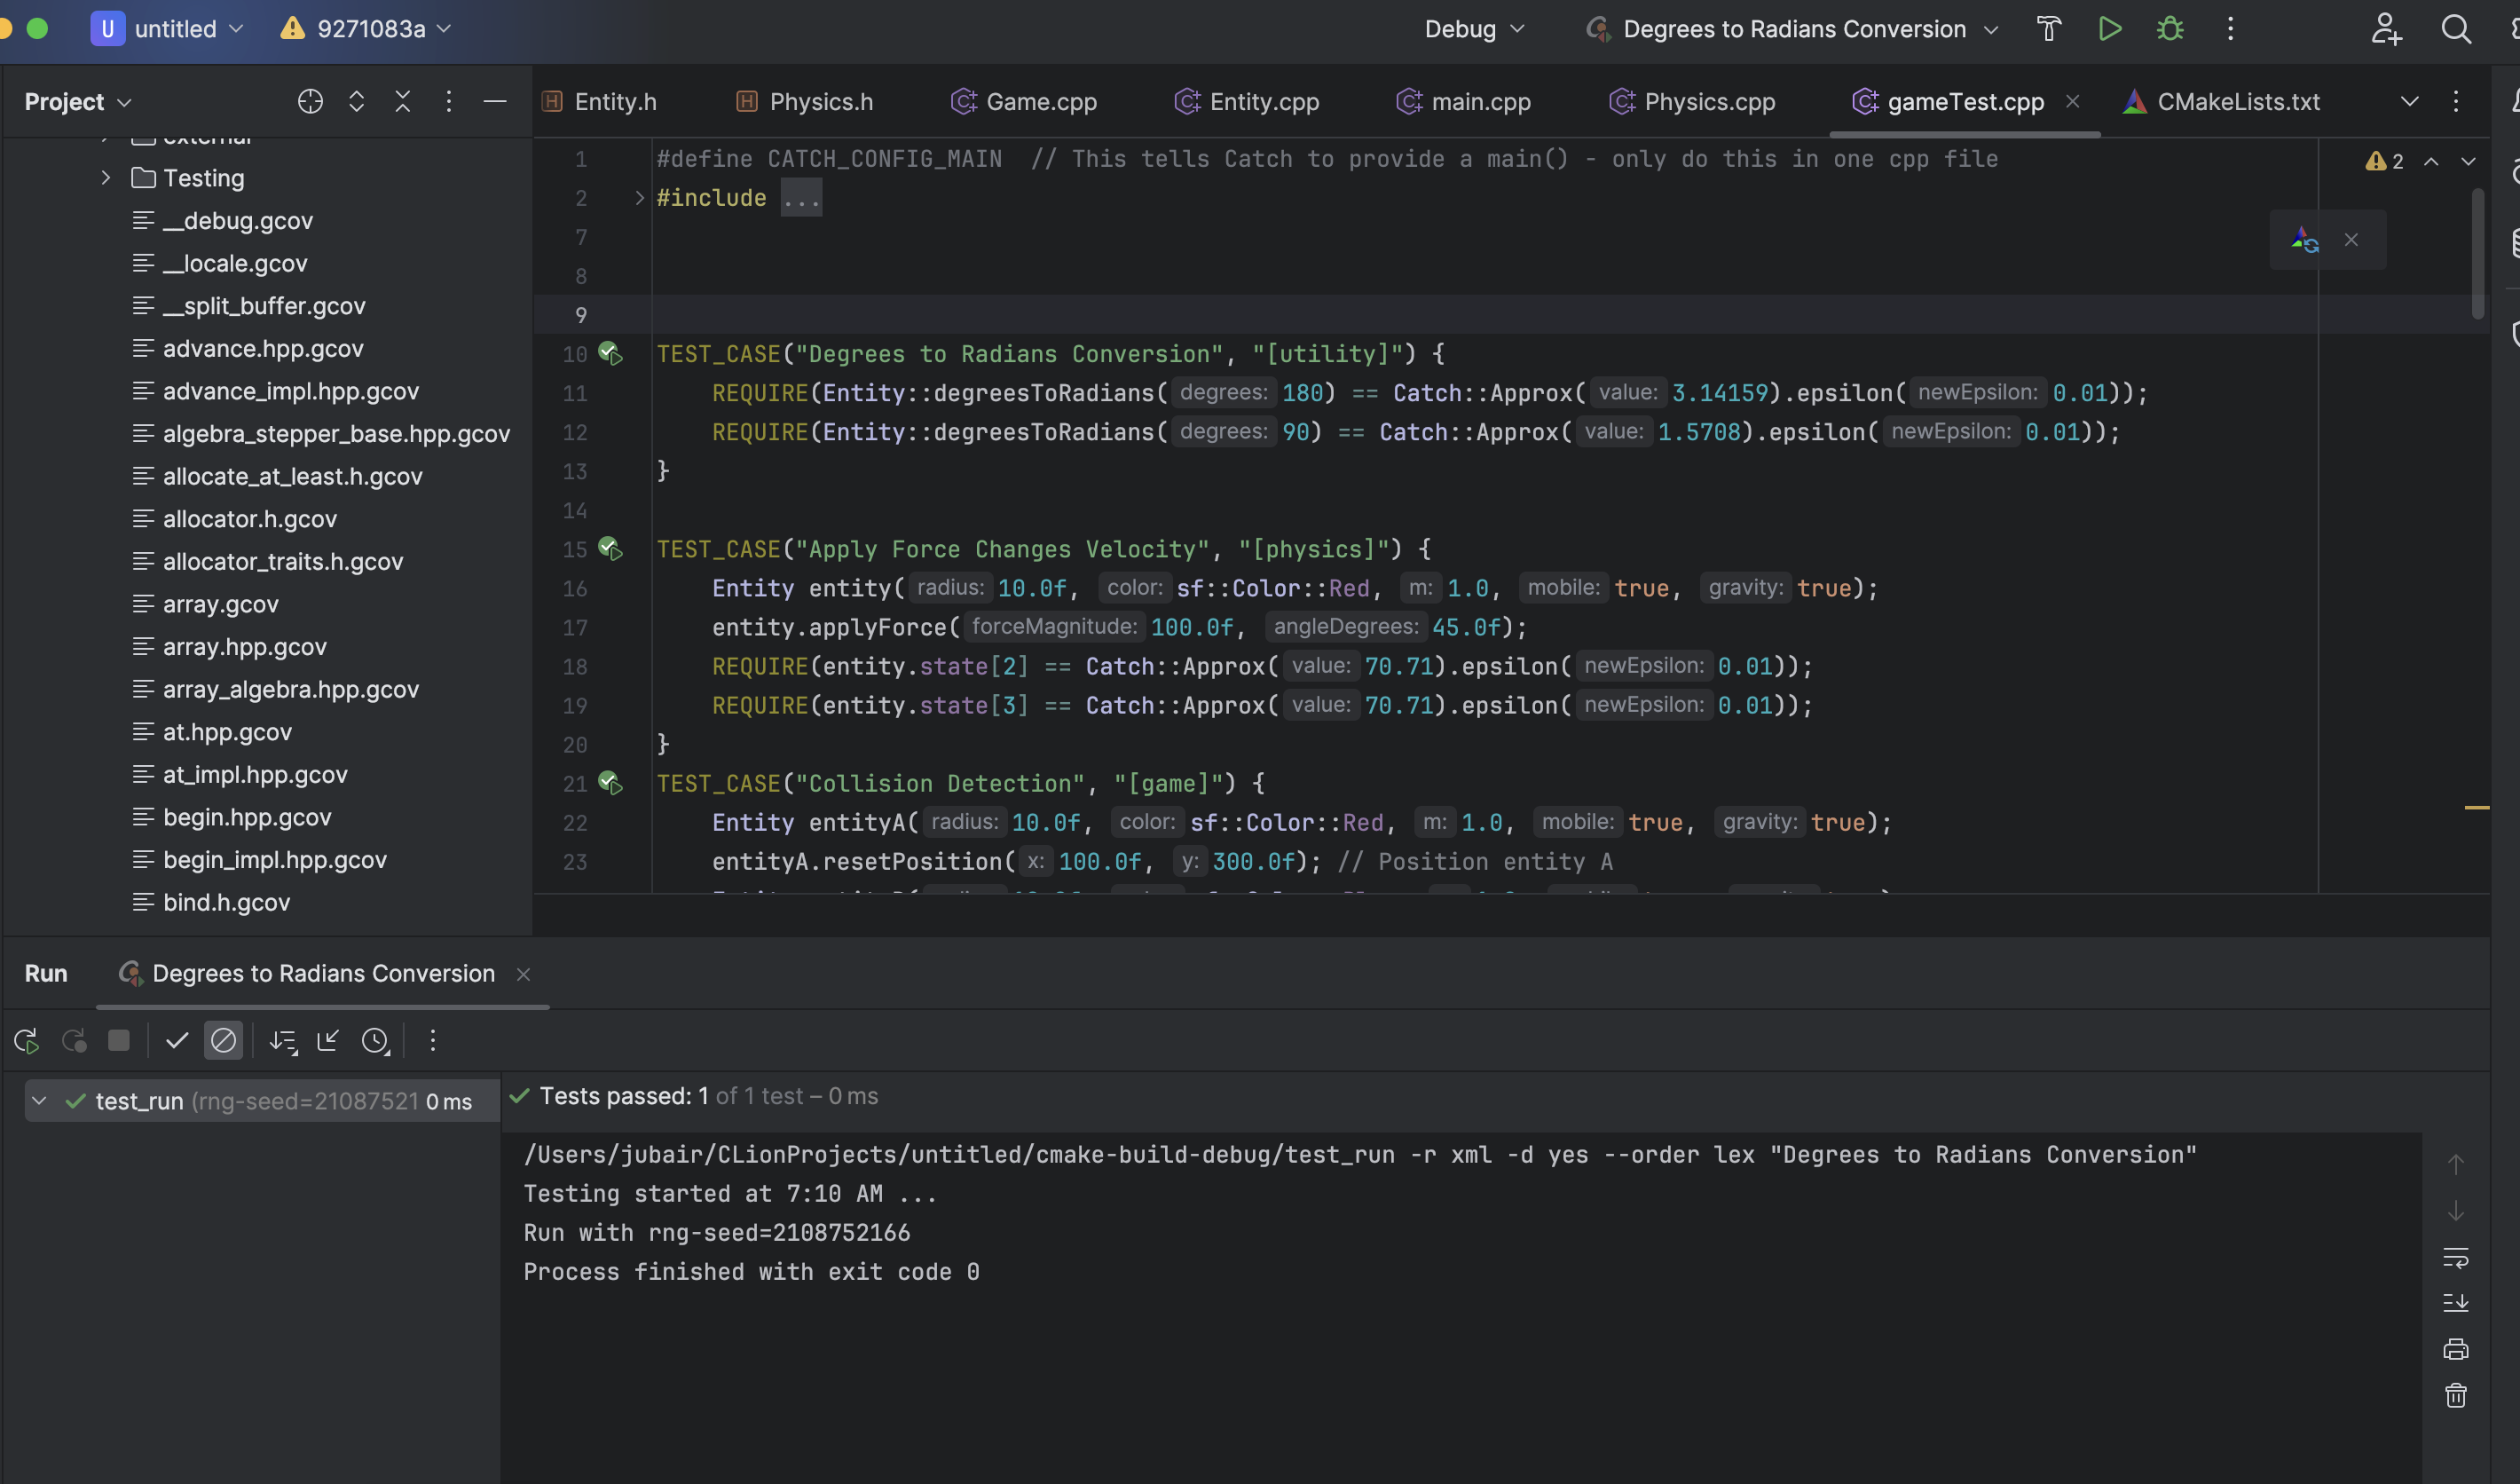
\includegraphics[width=\linewidth]{t1.png} % Replace path/to/your_image_1.png with the actual file path
    \caption{Visualization of test case 1 showing degrees to radians conversion.}
    \label{fig:test_case_1}
\end{figure}

\FloatBarrier
\subsection{Test Case 2: Apply Force Changes Velocity}

\begin{figure}[h!]
    \centering
    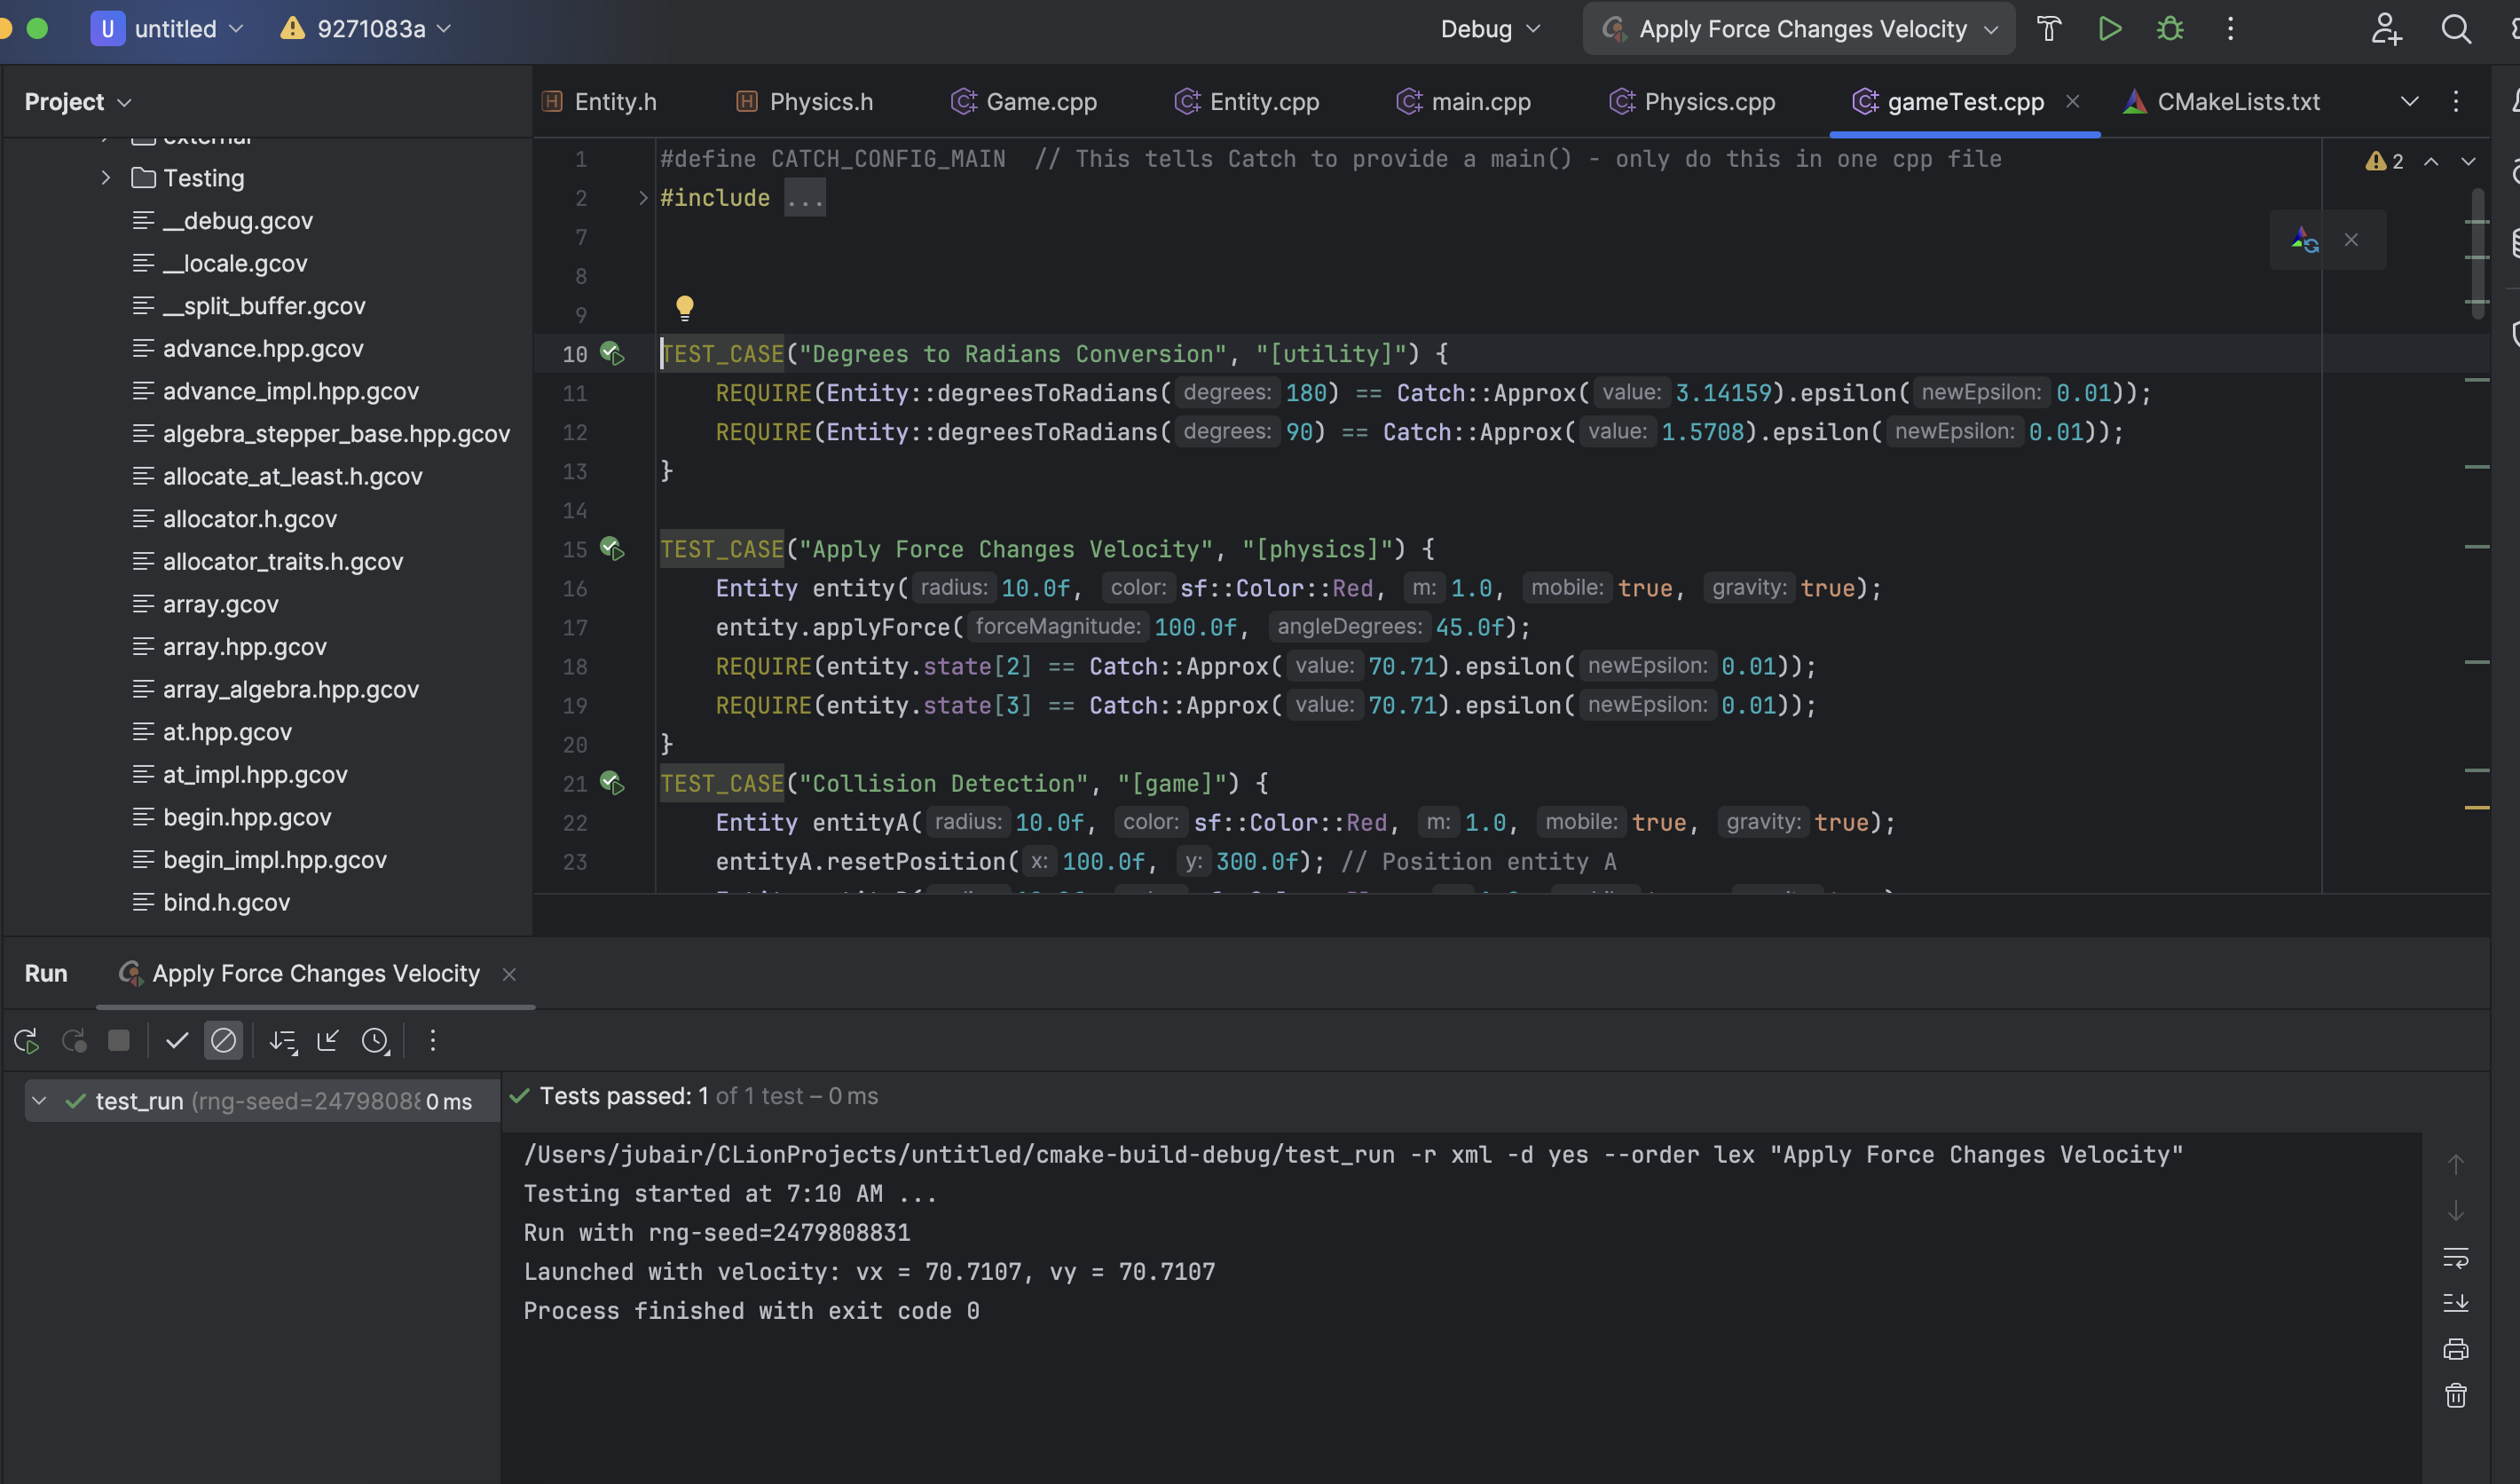
\includegraphics[width=\linewidth]{t2.png} % Replace path/to/your_image_2.png with the actual file path
    \caption{Visualization of test case 2 showing how applying force changes entity velocity.}
    \label{fig:test_case_2}
\end{figure}
\FloatBarrier
\subsection{Test Case 3: Collision Detection}

\begin{figure}[h!]
    \centering
    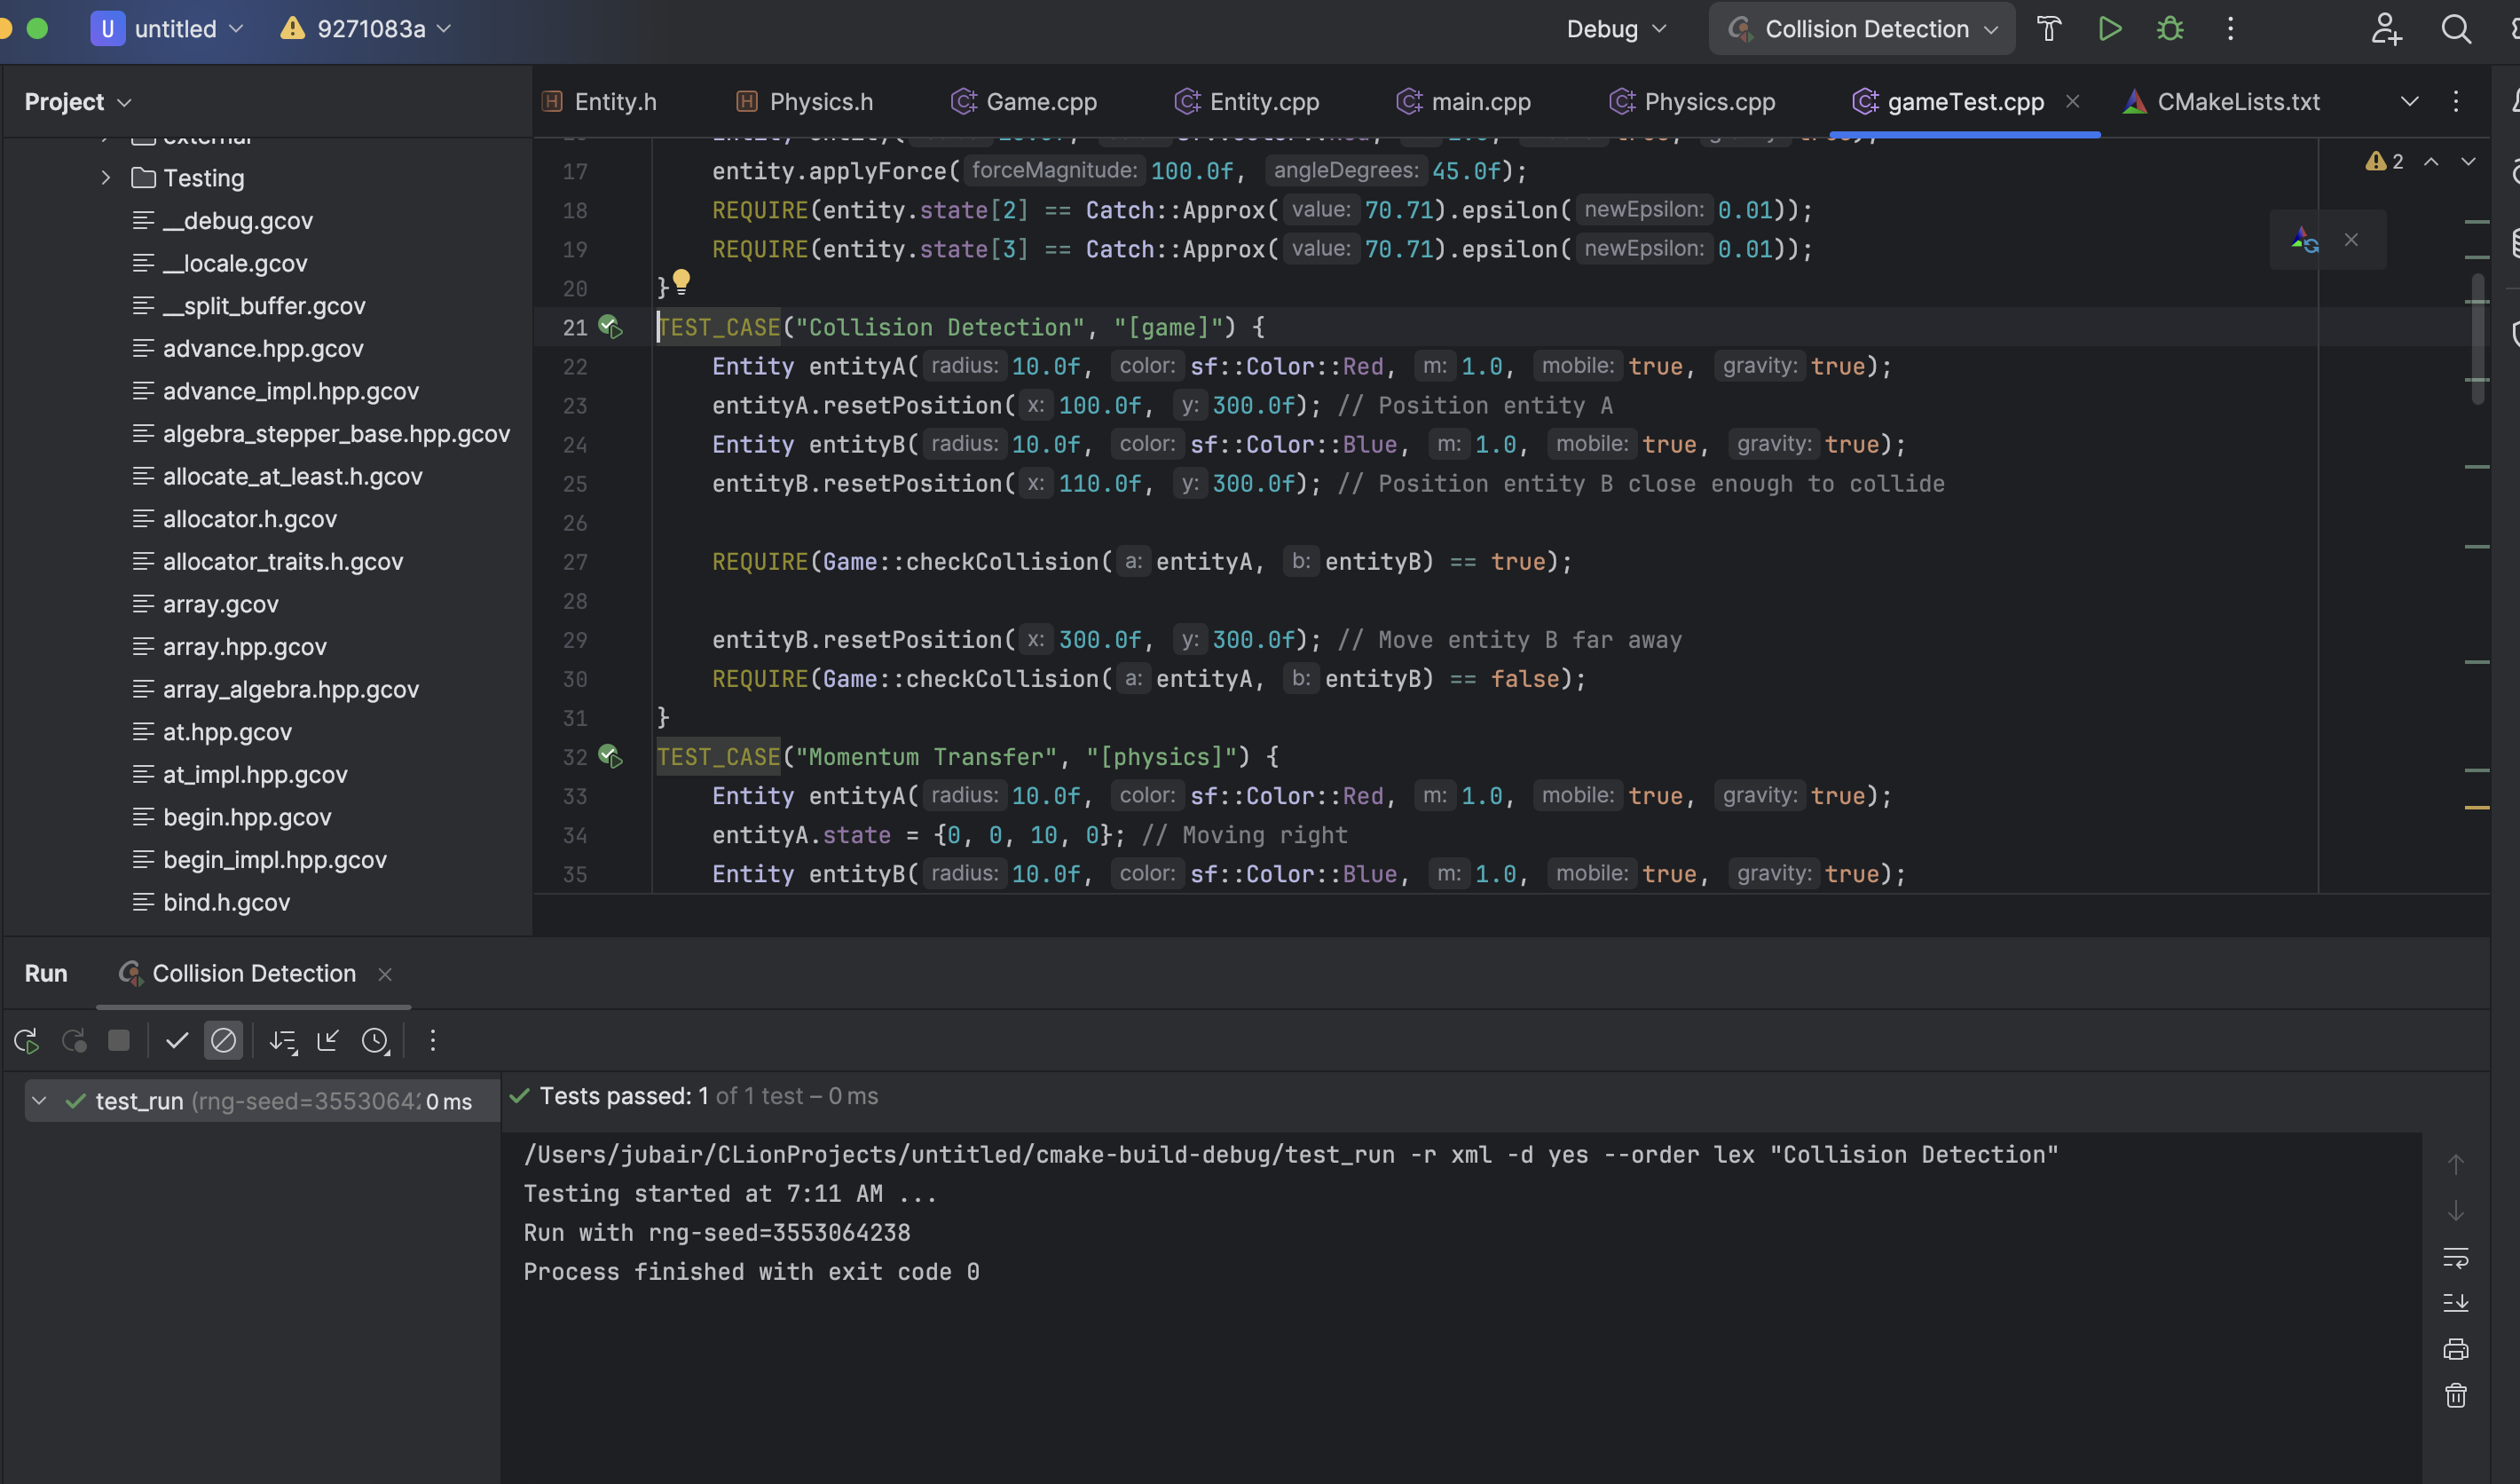
\includegraphics[width=\linewidth]{t3.png} 
    \caption{Visualization of test case 3 showing collision detection between entities.}
    \label{fig:test_case_3}
\end{figure}
\FloatBarrier
\subsection{Test Case 4: Momentum Transfer}

\begin{figure}[h!]
    \centering
    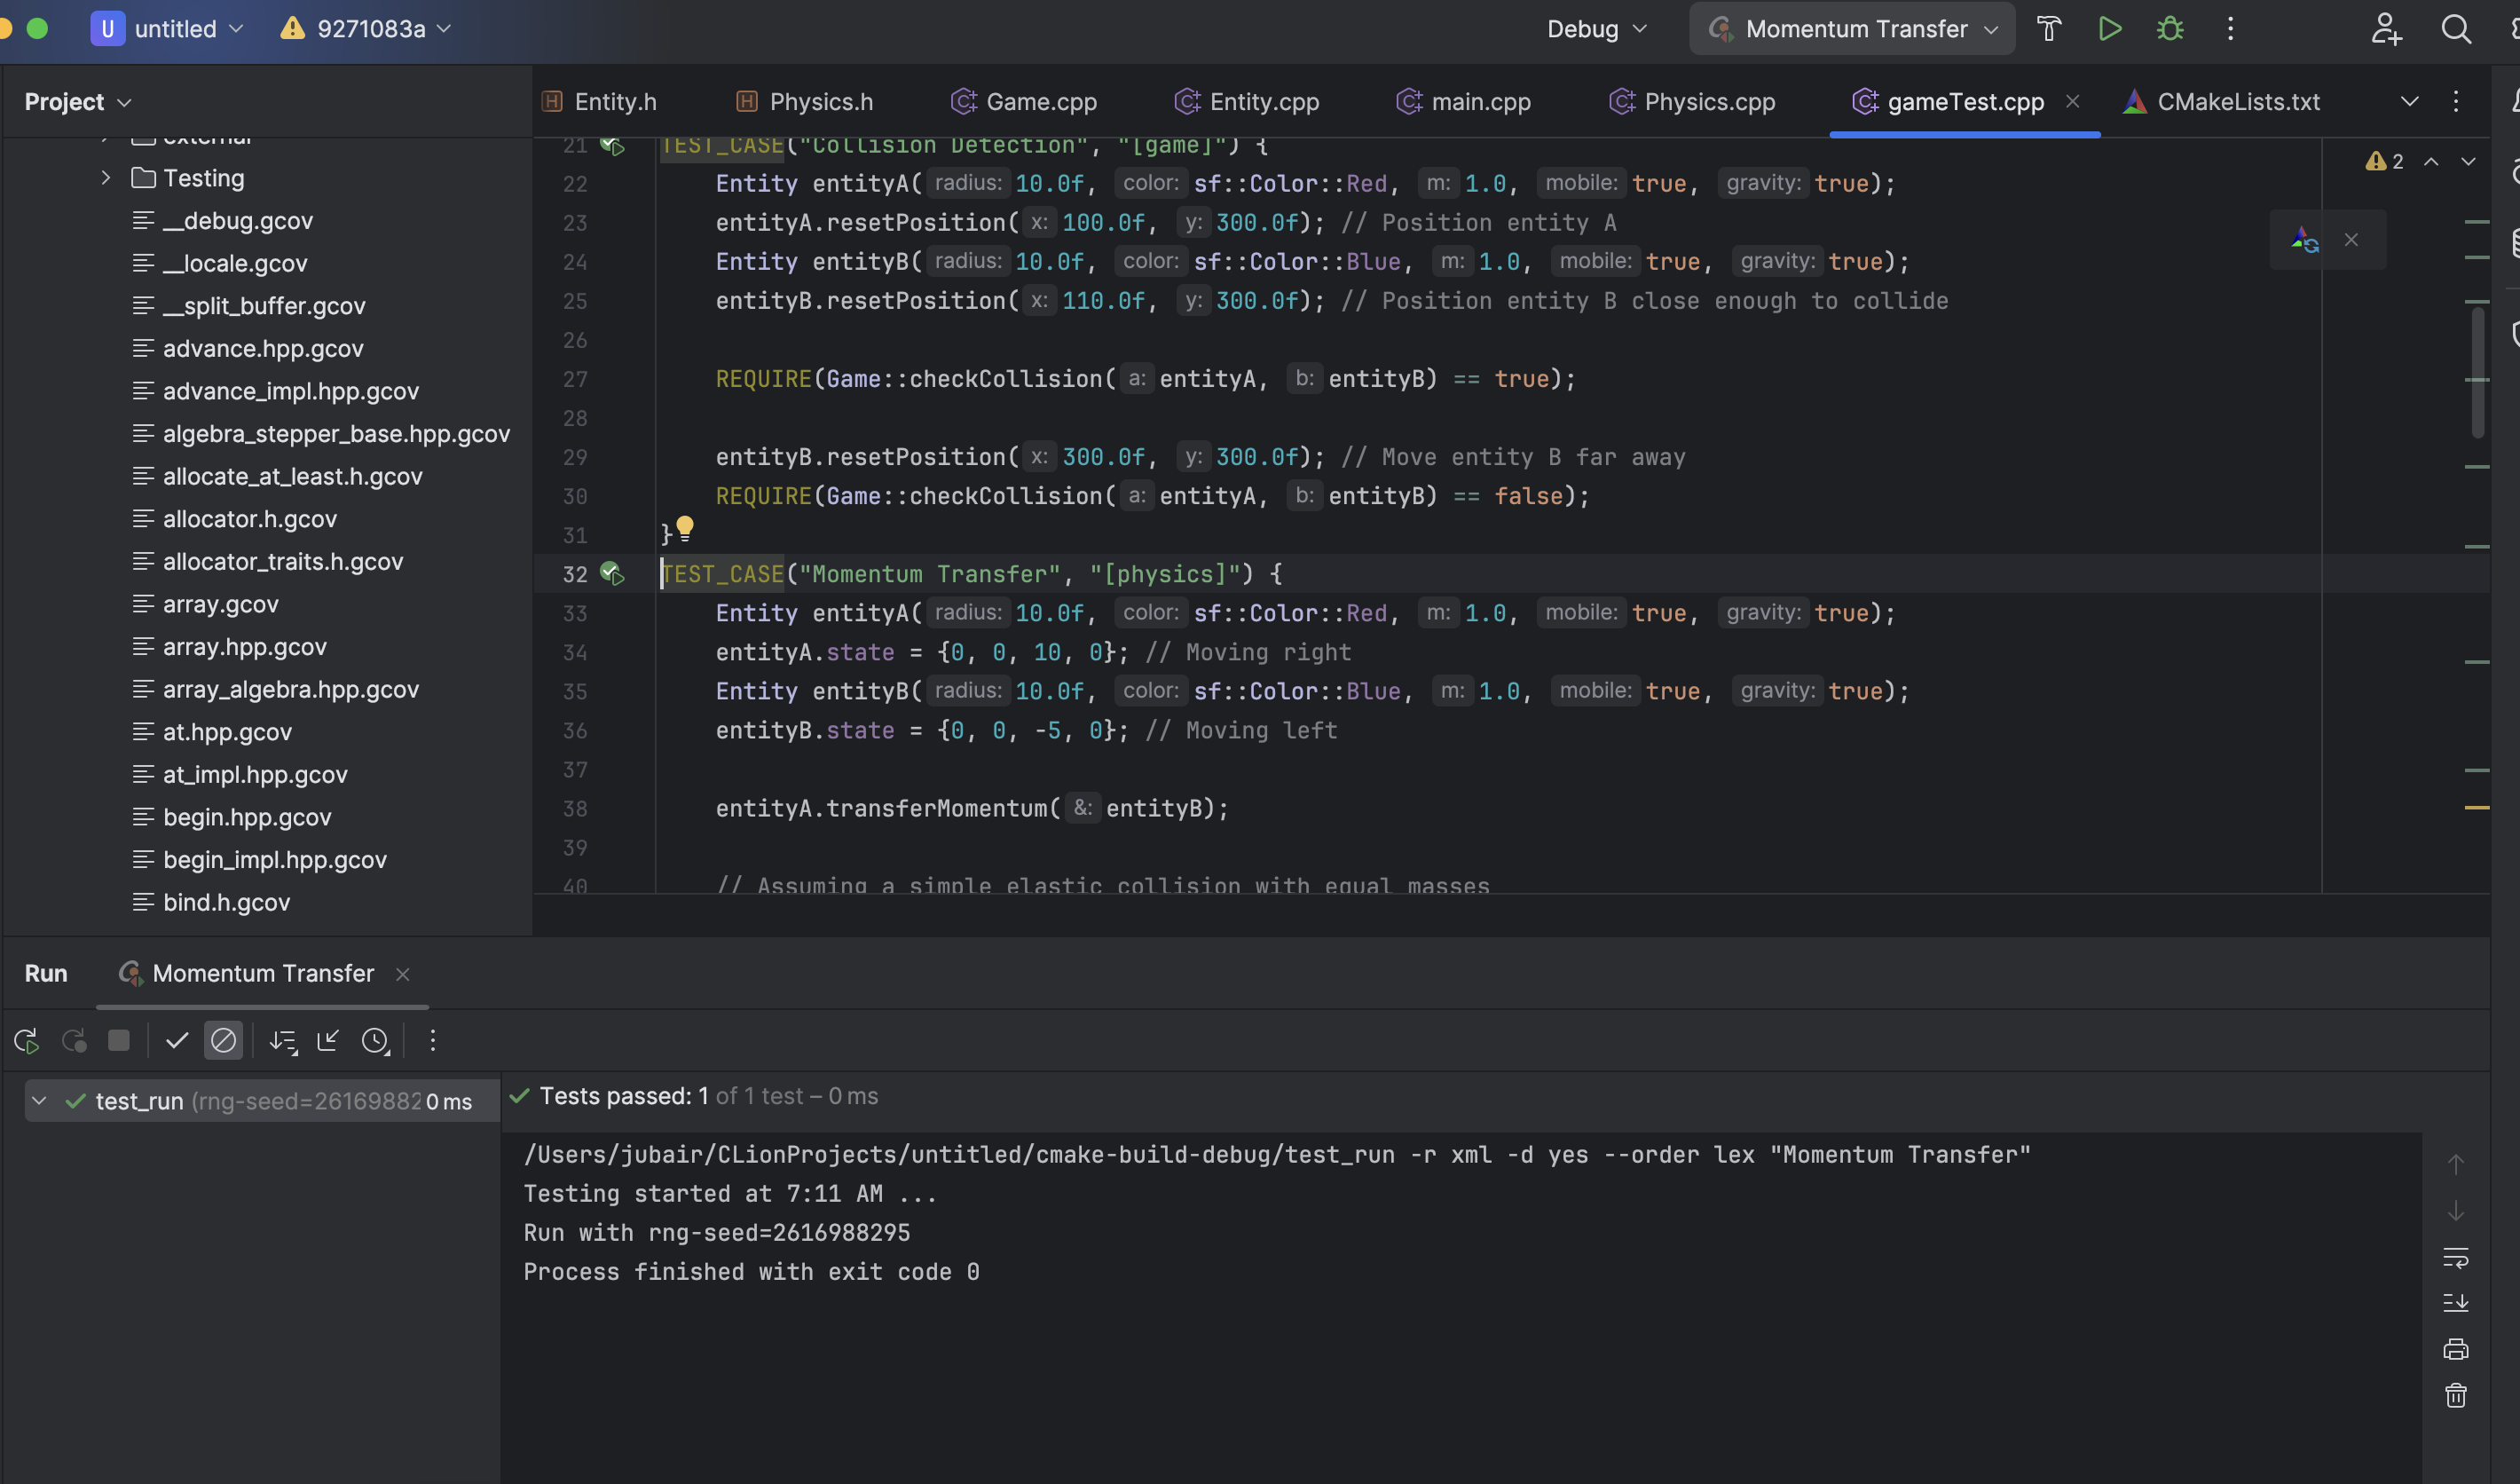
\includegraphics[width=\linewidth]{t4.png} 
    \caption{Visualization of test case 4 showing collision detection between entities.}
    \label{fig:test_case_4}
\end{figure}
\FloatBarrier
\subsection{Test Case 4: Game Reset Mechanism}

\begin{figure}[h!]
    \centering
    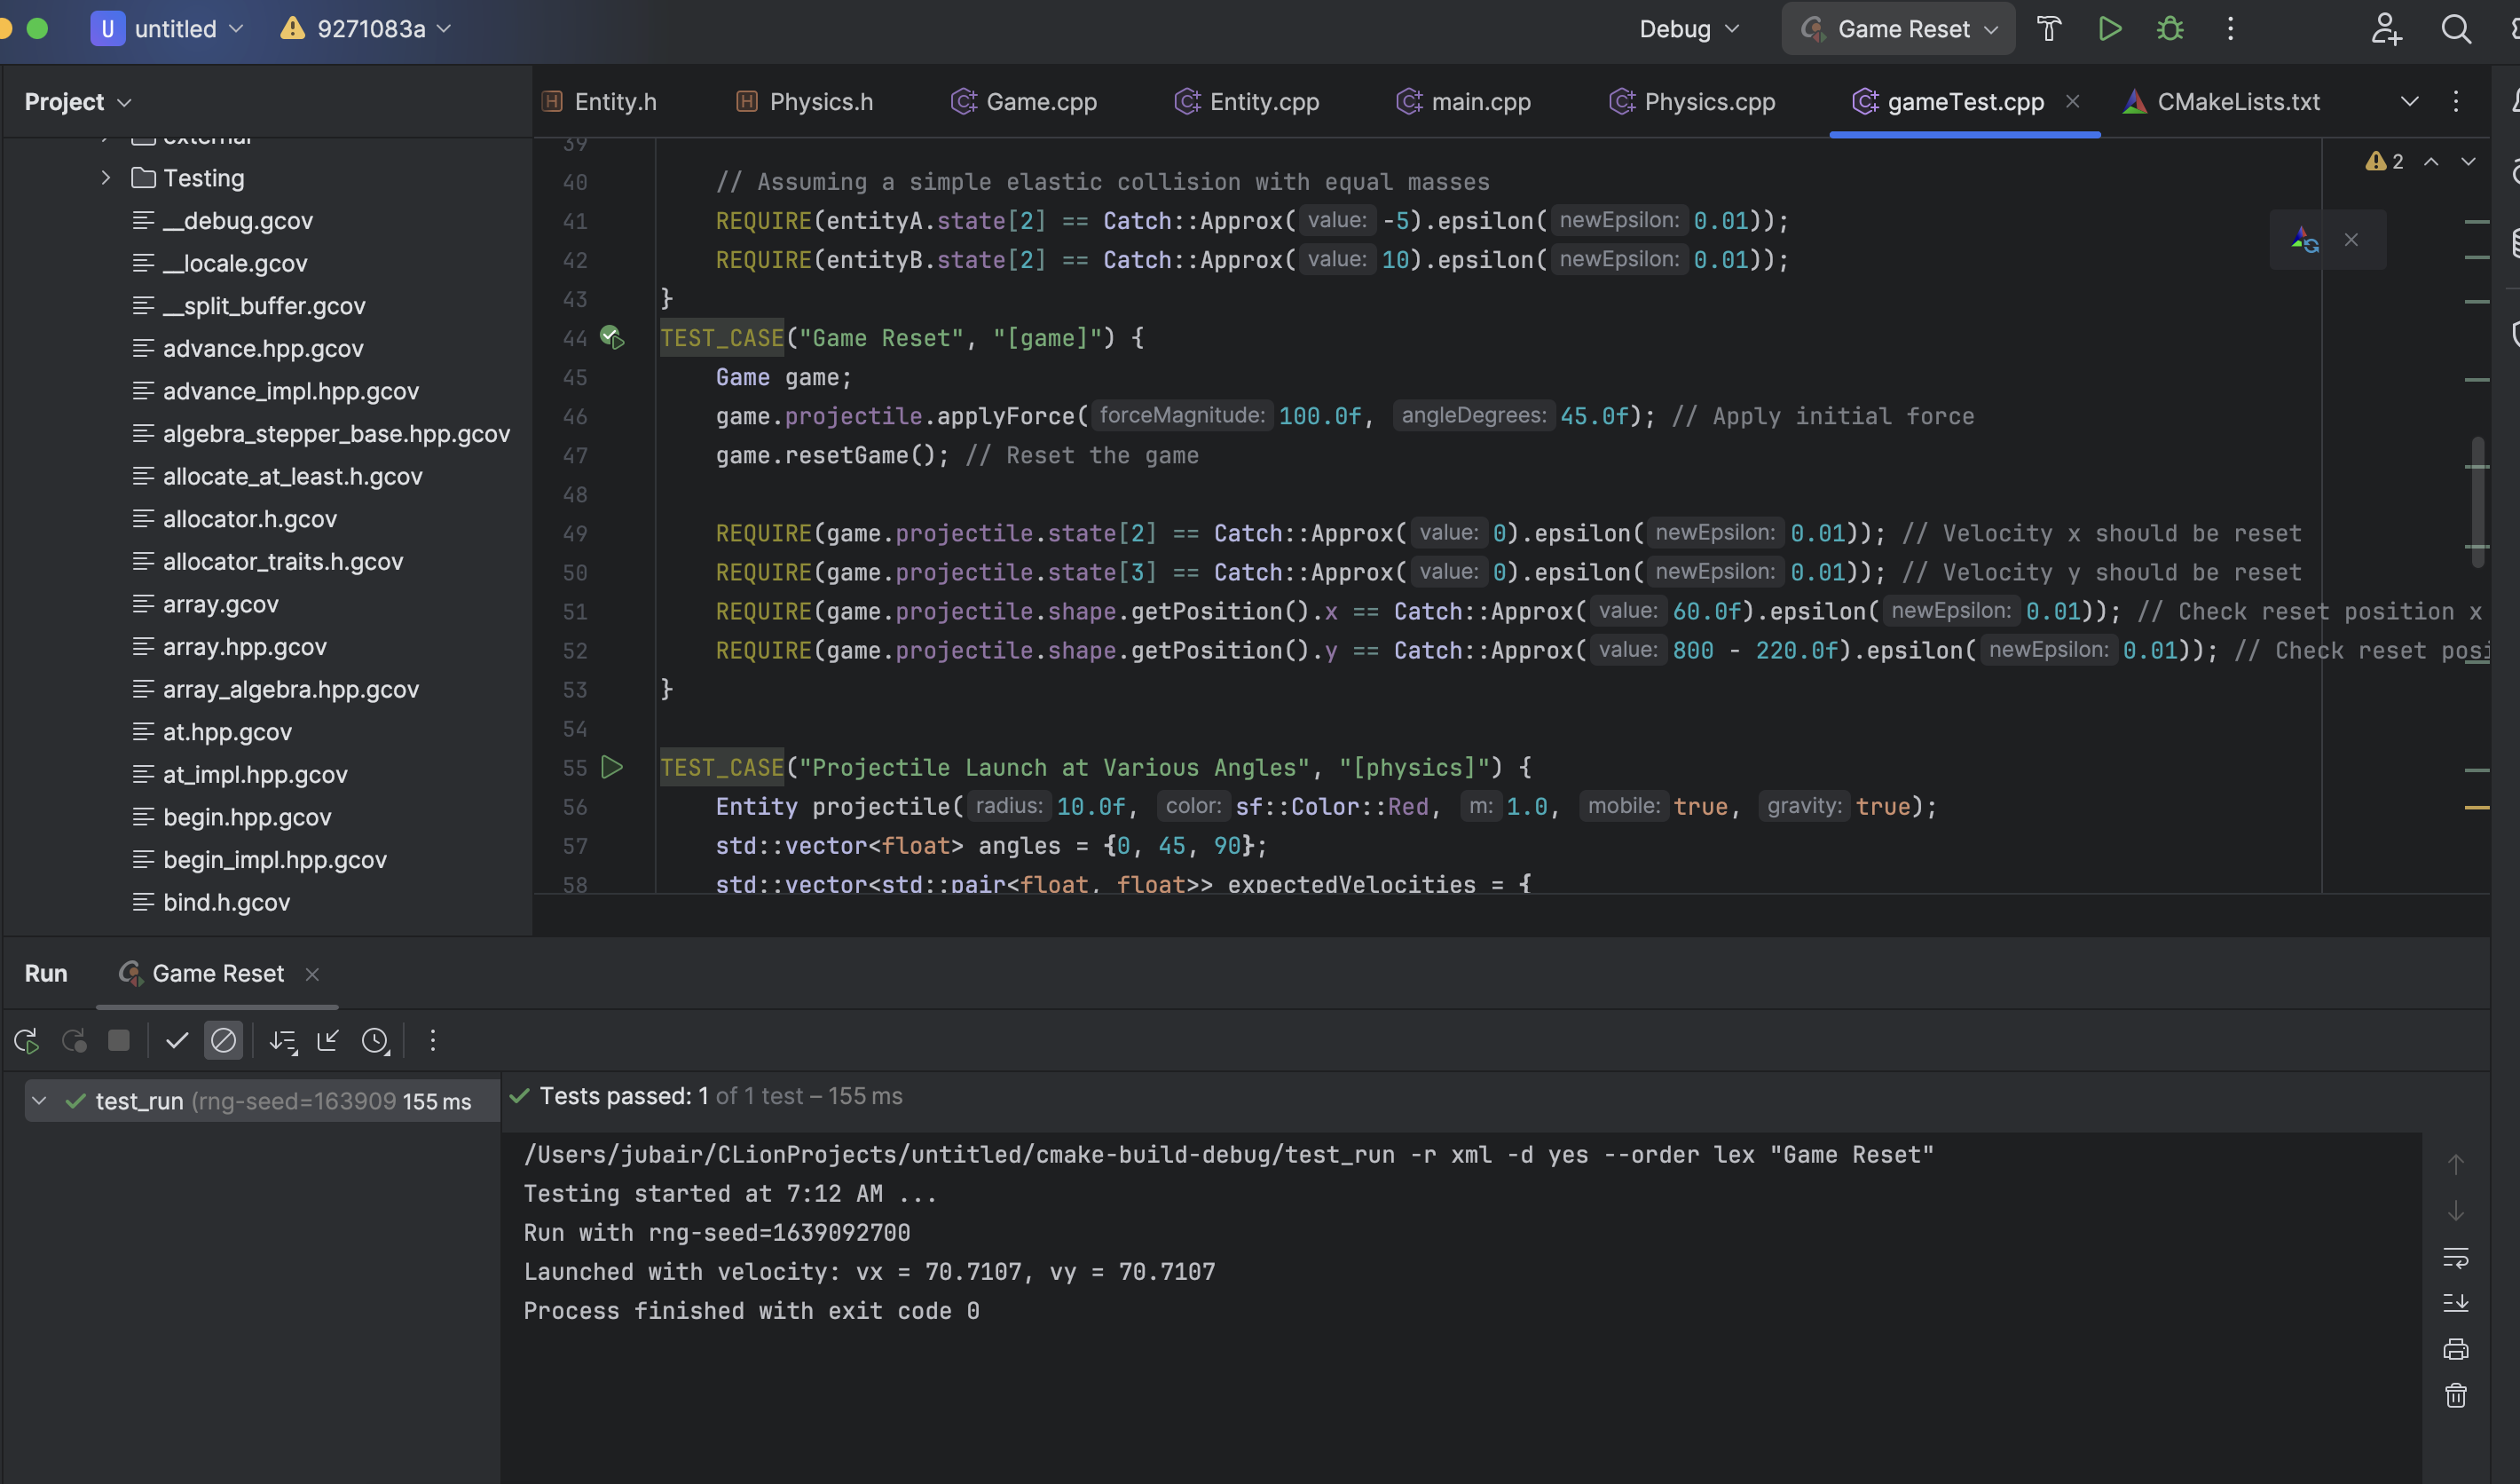
\includegraphics[width=\linewidth]{t5.png} 
    \caption{Visualization of test case 5 showing the game reset mechanism in action.}
    \label{fig:test_case_5}
\end{figure}
\FloatBarrier
\subsection{Test Case 5: Projectile Launch at Various Angles}

\begin{figure}[h!]
    \centering
    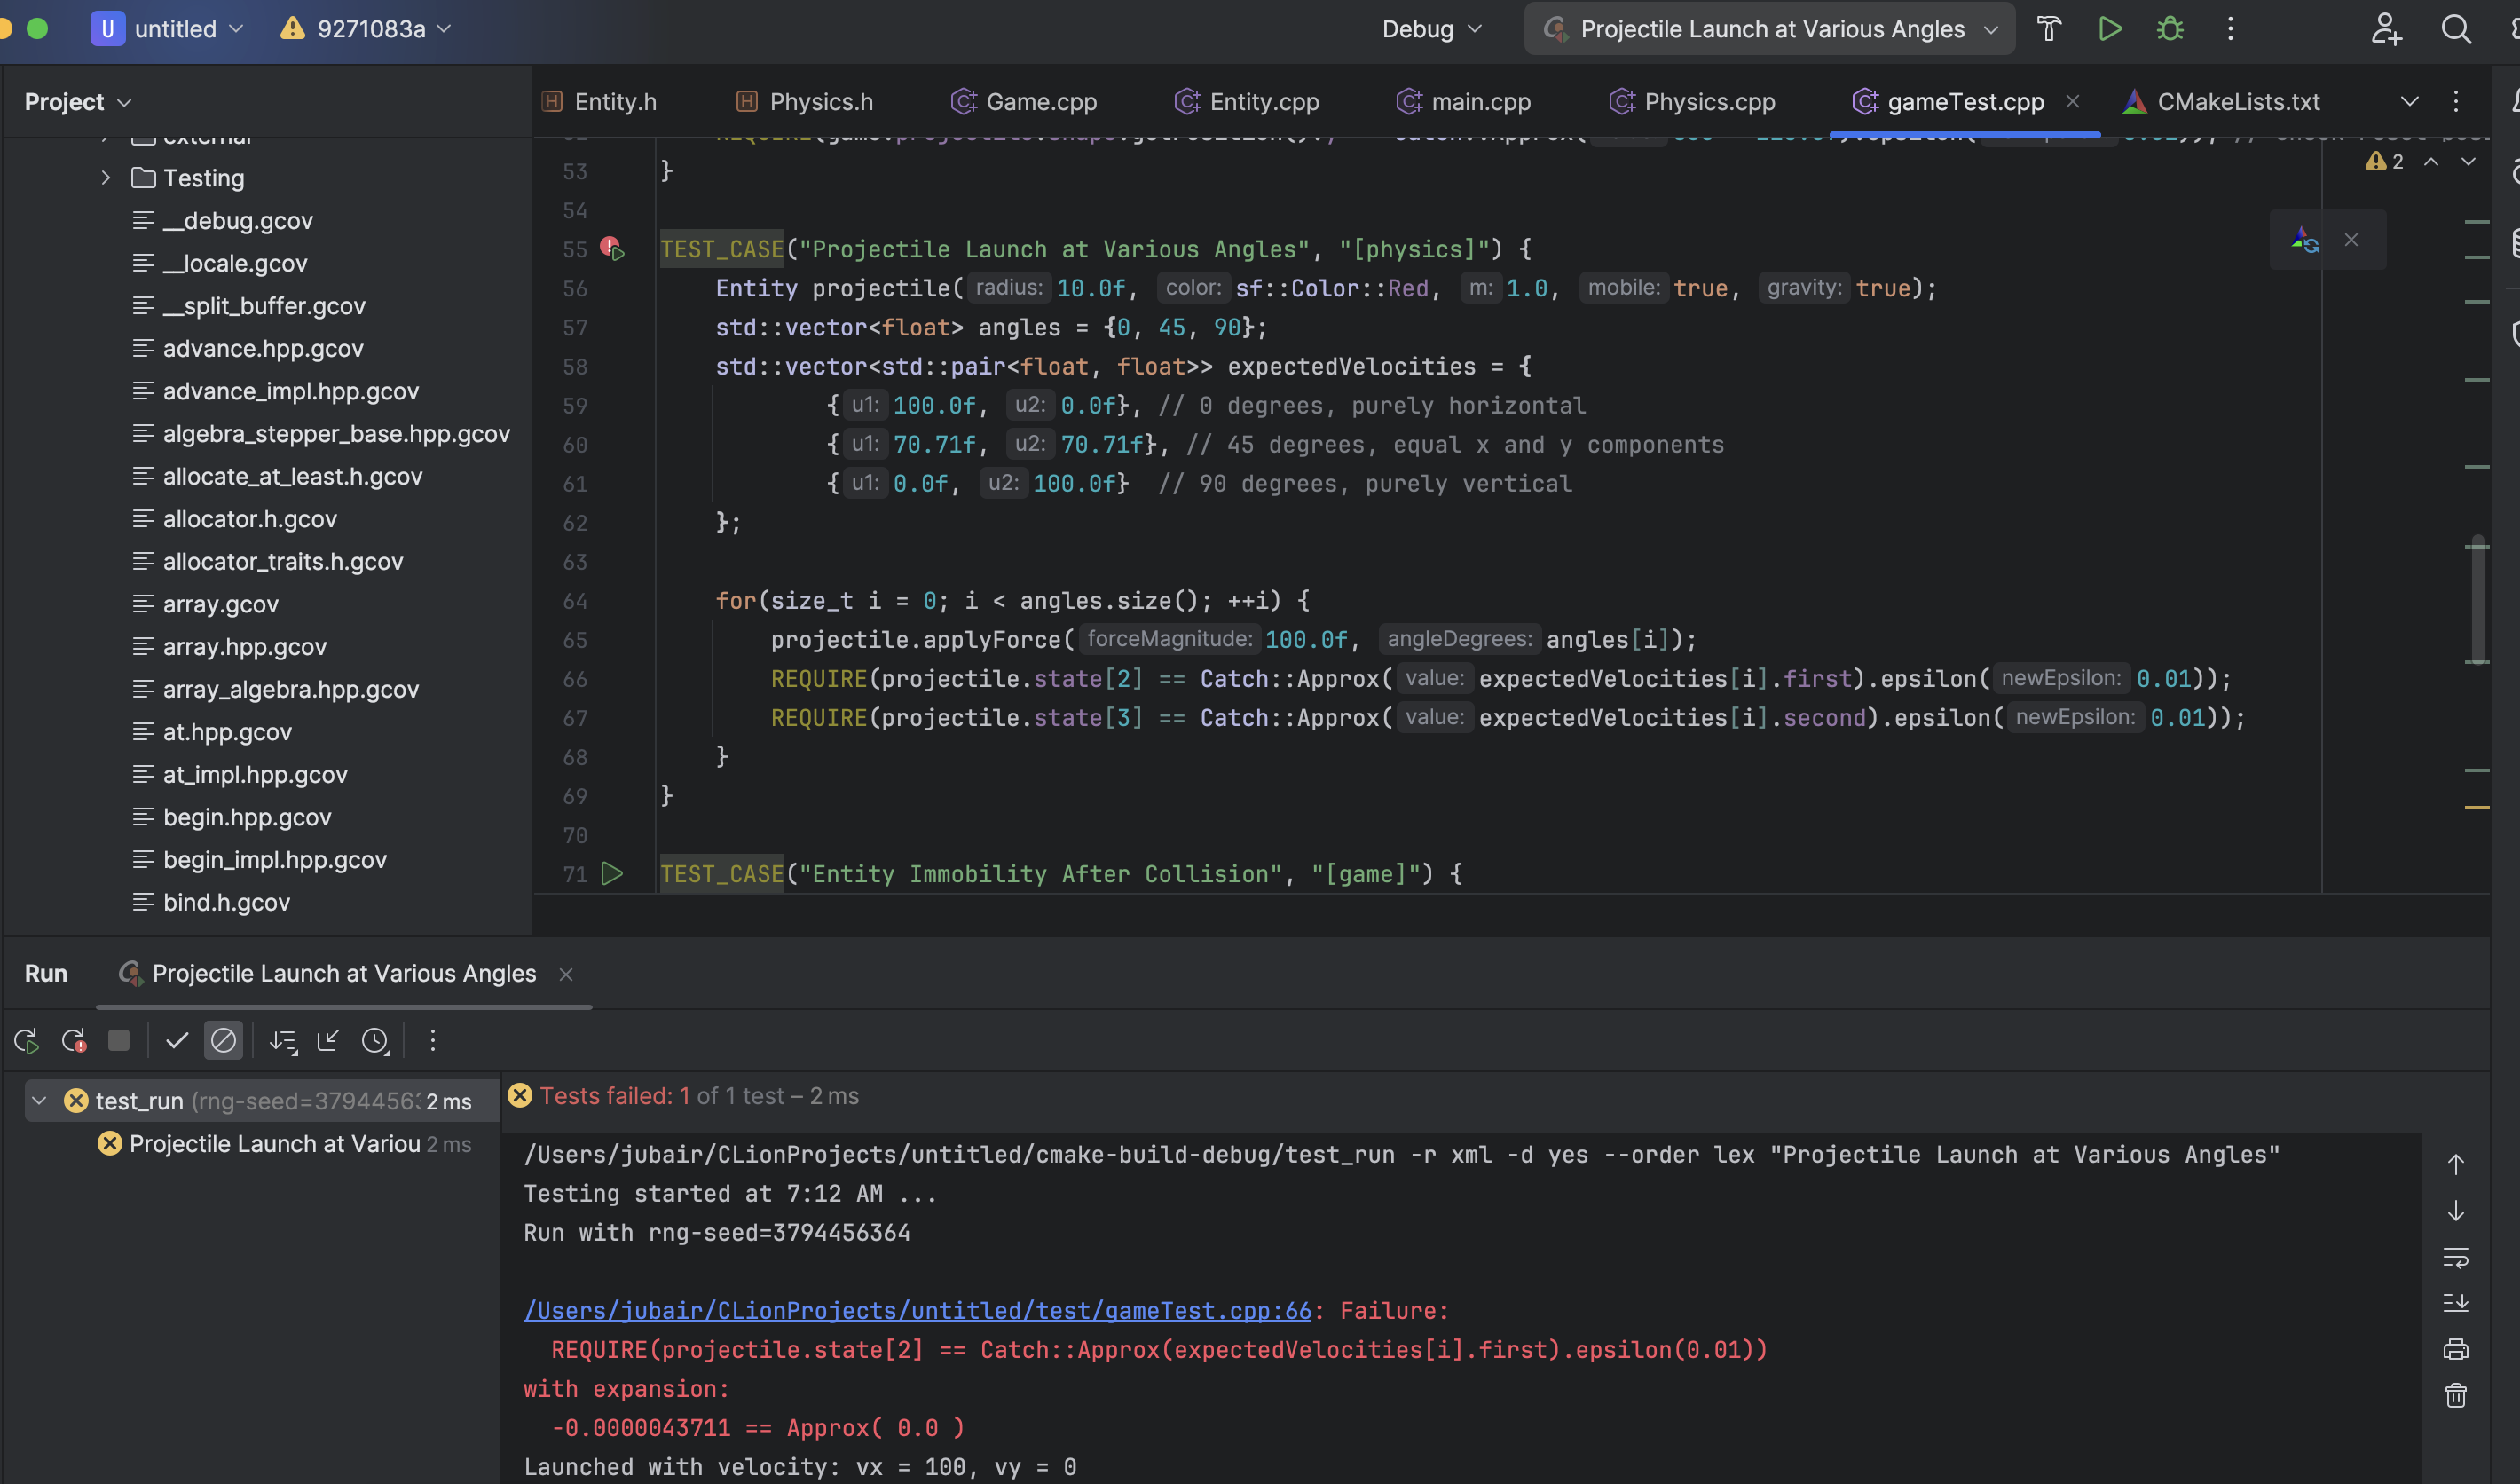
\includegraphics[width=\linewidth]{t6.png} 
    \caption{Visualization of test case 6 demonstrating projectile launch at various angles.}
    \label{fig:test_case_6}
\end{figure}
\FloatBarrier
\subsection{Test Case 6: Entity Immobility After Collision}

\begin{figure}[h!]
    \centering
    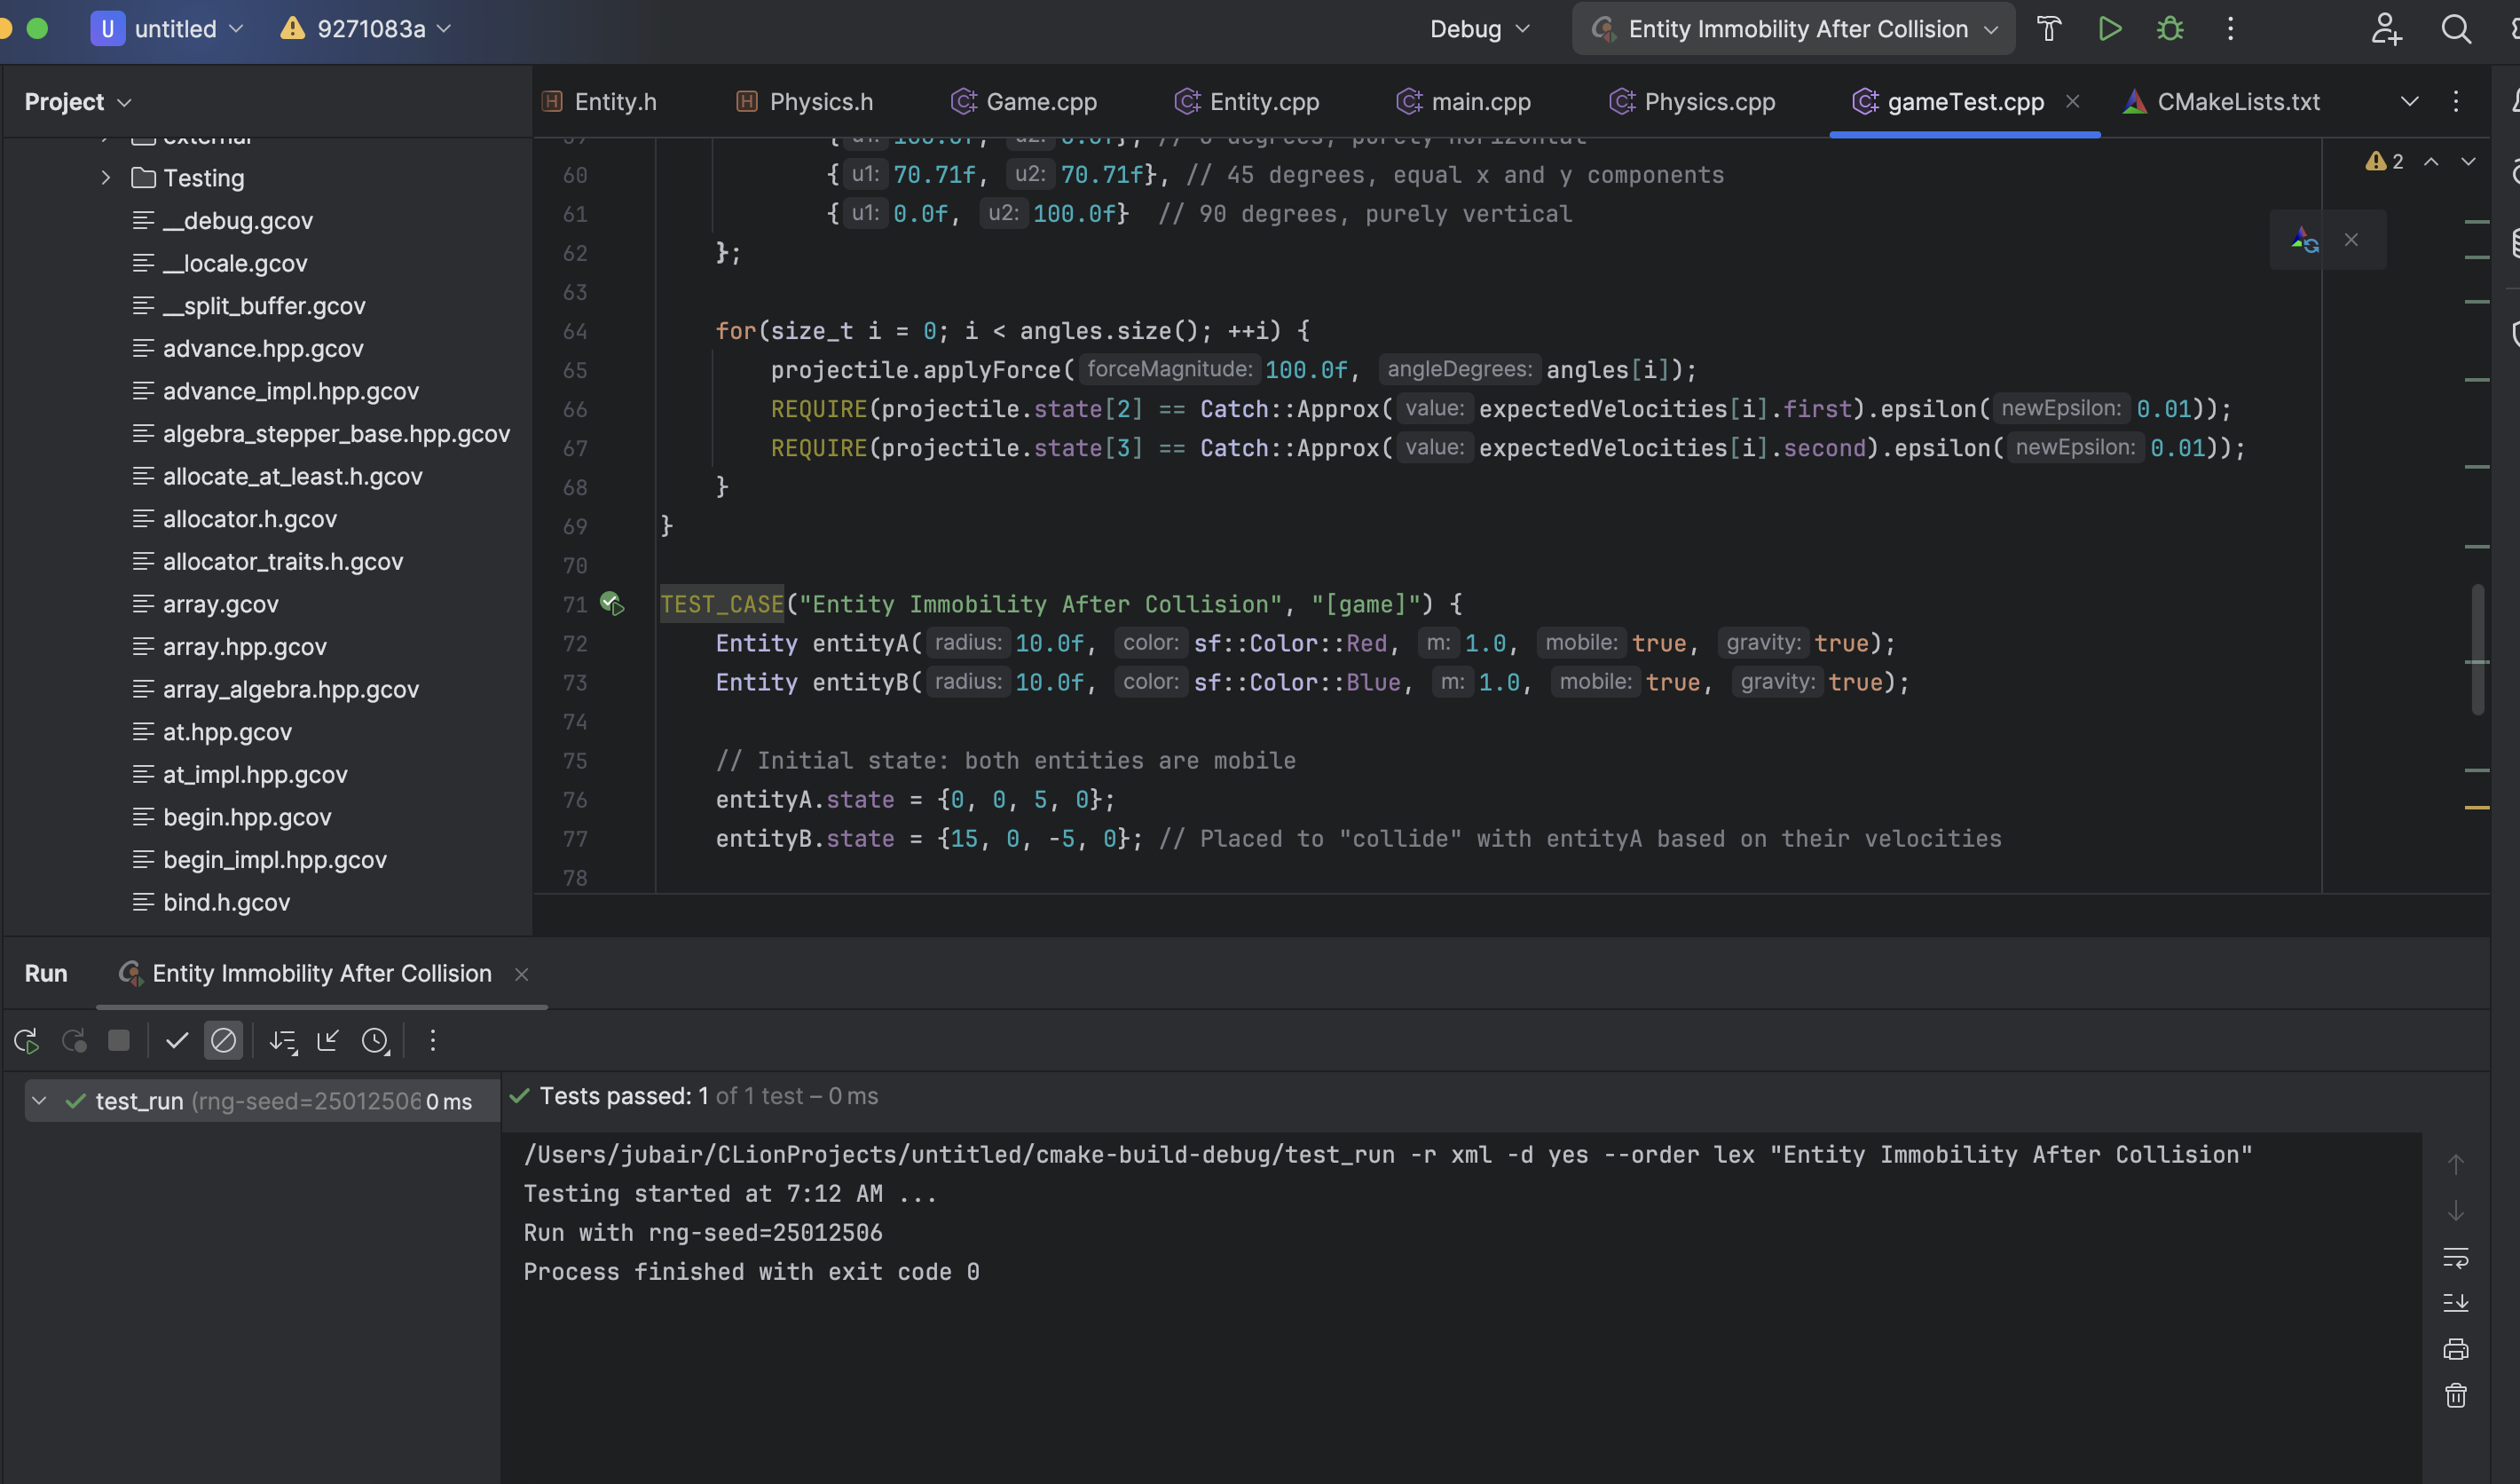
\includegraphics[width=\linewidth]{t7.png} 
    \caption{Visualization of test case 7 showing entities becoming immobile after collision.}
    \label{fig:test_case_7}
\end{figure}
\FloatBarrier
\subsection{Test Case 7: Entity Gravity Effect}

\begin{figure}[h!]
    \centering
    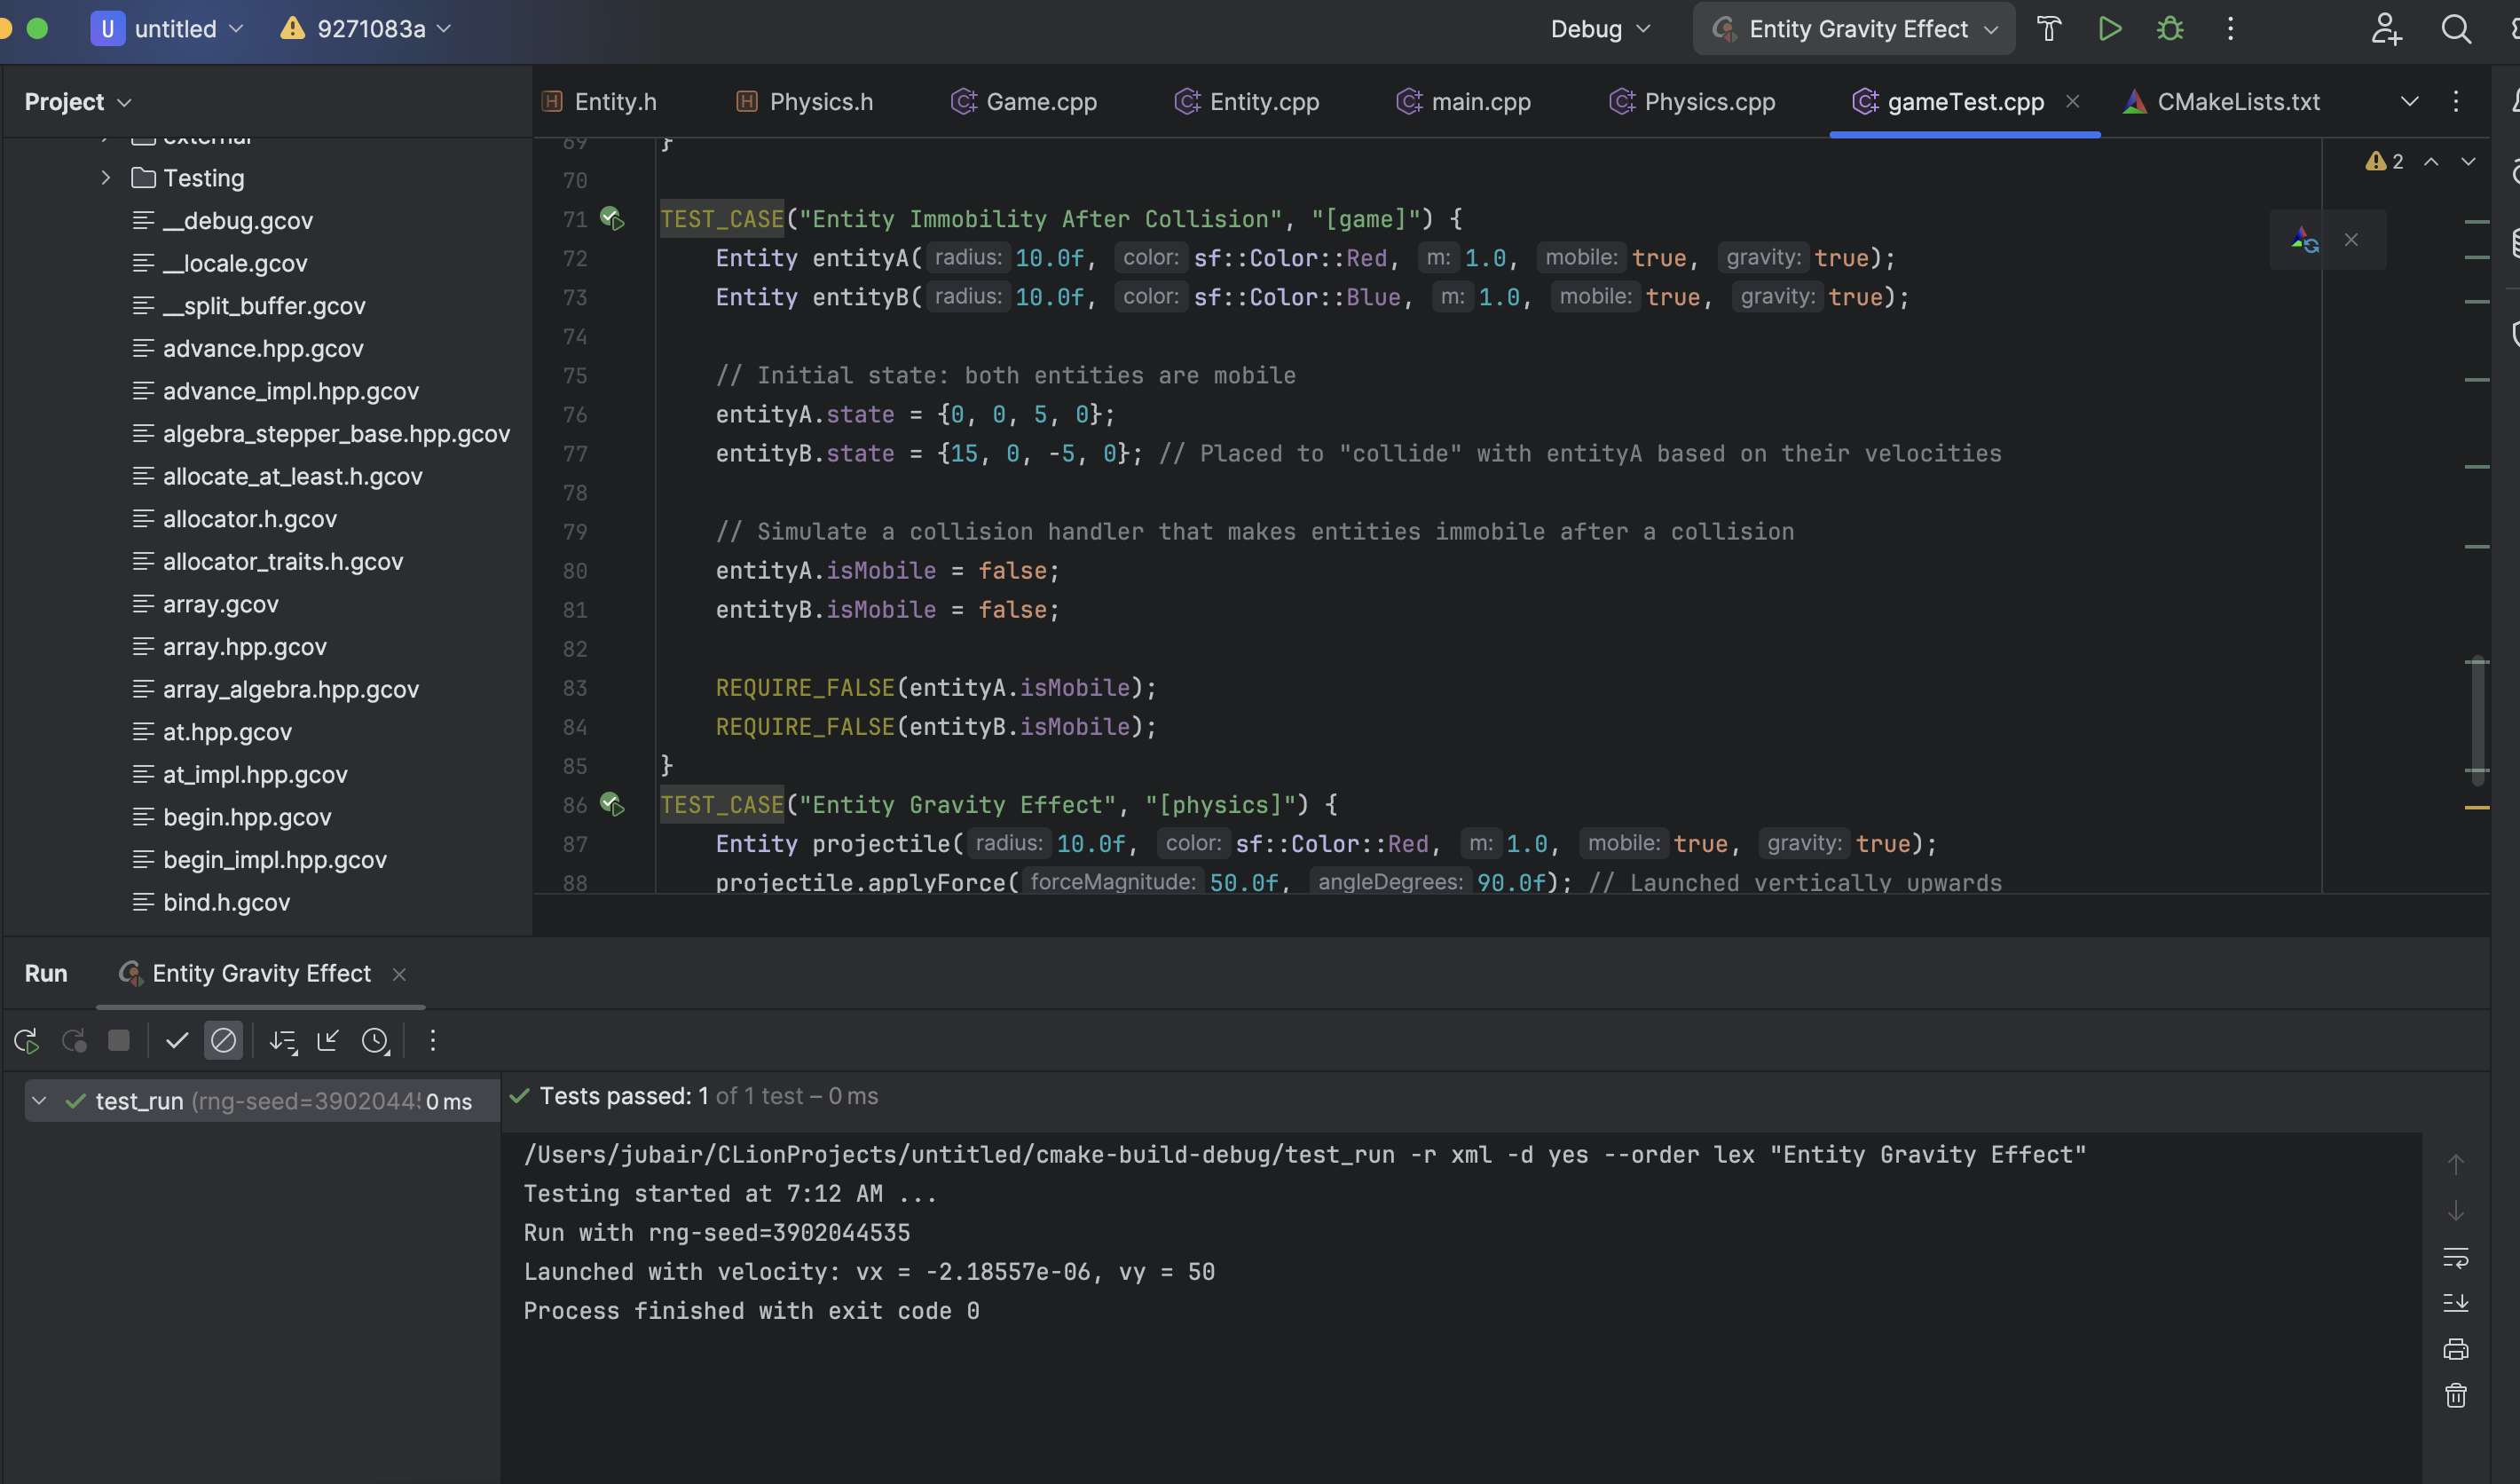
\includegraphics[width=\linewidth]{t8.png} 
    \caption{Visualization of test case 8 illustrating the effect of gravity on an entity.}
    \label{fig:test_case_8}
\end{figure}

\FloatBarrier

\section{Code Coverage Metrics}

\subsection{Coverage for Game.cpp}

\begin{figure}[h!]
    \centering
    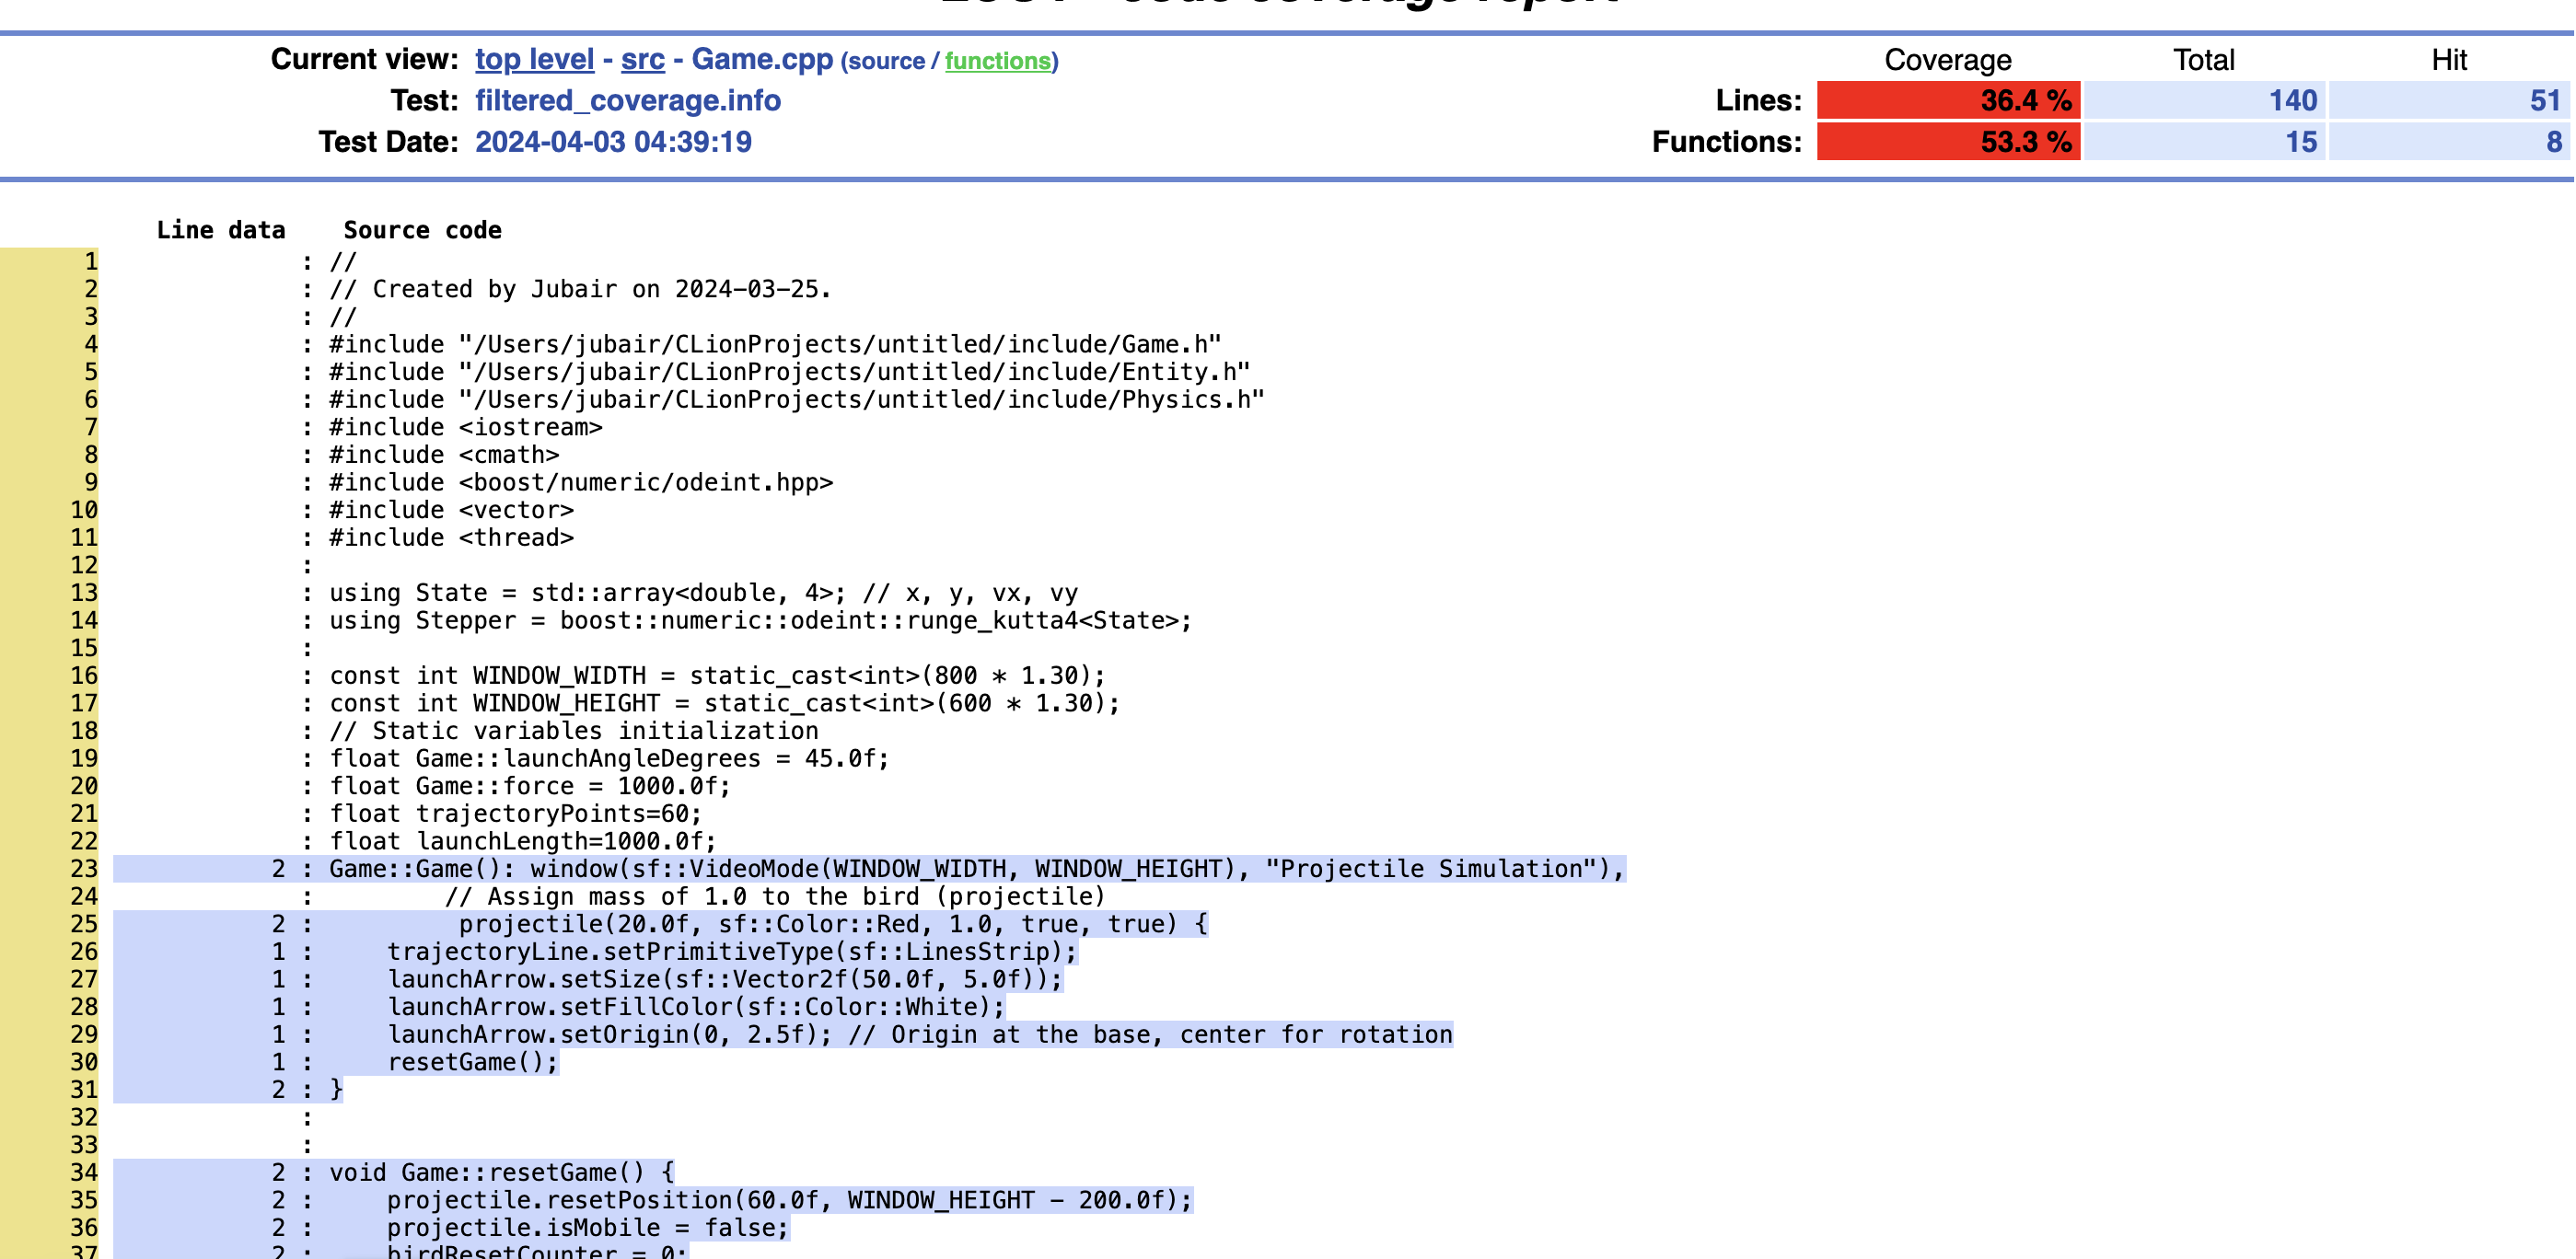
\includegraphics[width=\linewidth]{gamecls.png}
    \caption{Test coverage report for Game.cpp, showing line coverage.}
    \label{fig:game_cpp_line_coverage}
\end{figure}

\begin{figure}[h!]
    \centering
    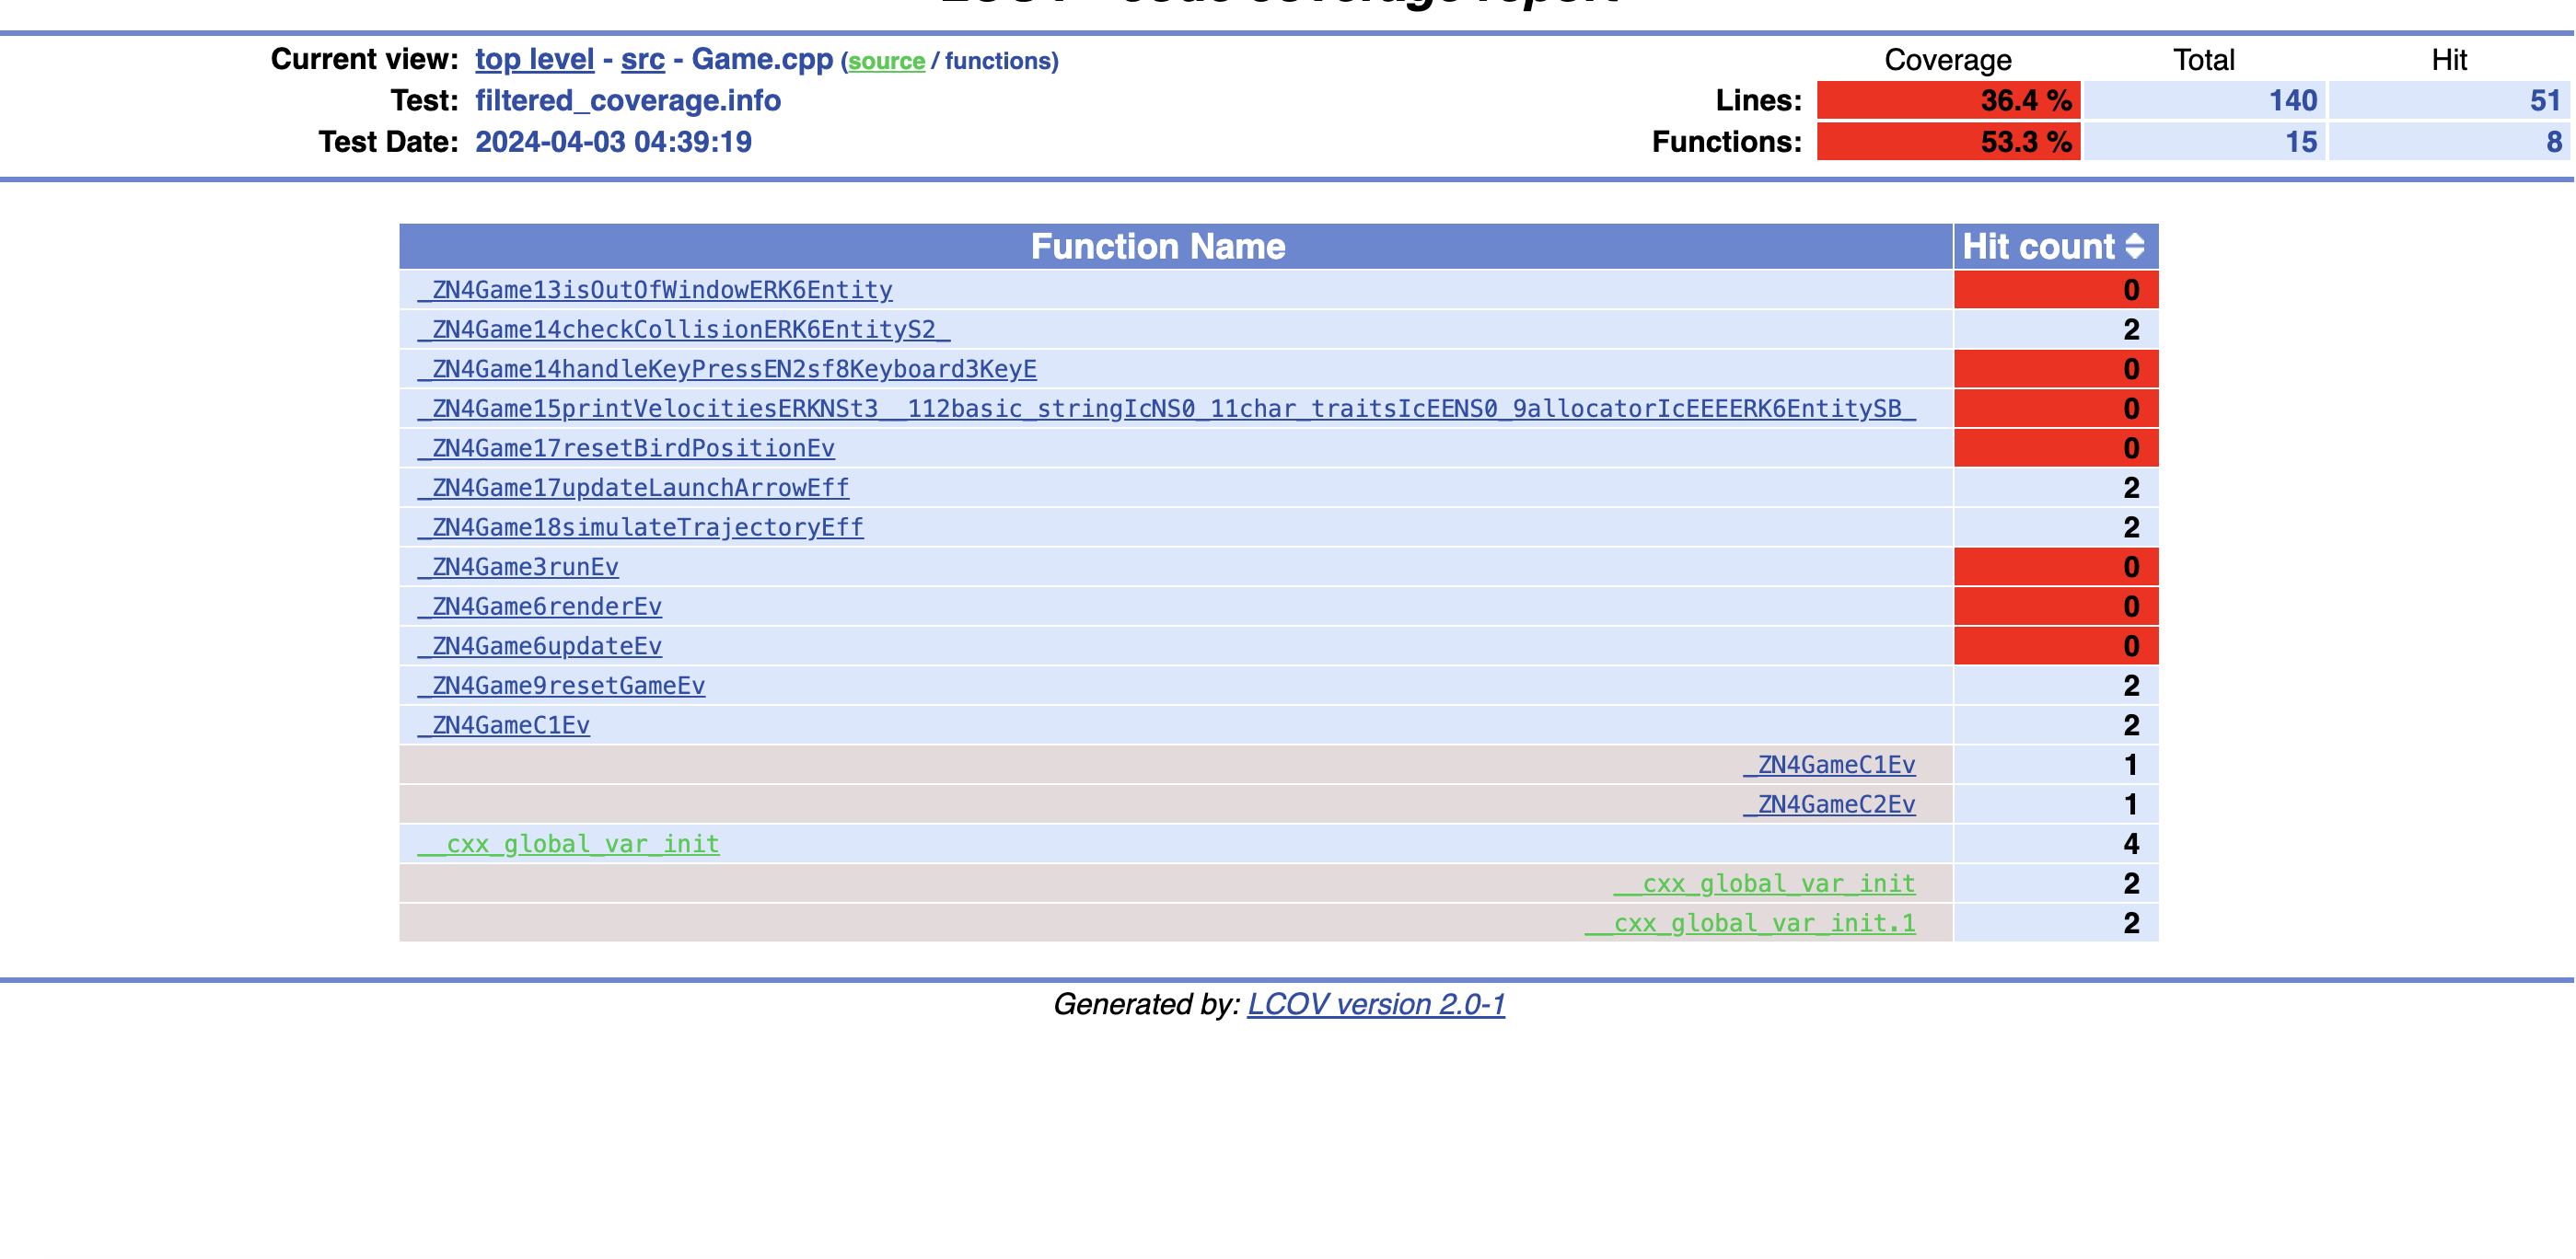
\includegraphics[width=\linewidth]{gamecf.png}
    \caption{Test coverage report for Game.cpp, showing function coverage.}
    \label{fig:game_cpp_function_coverage}
\end{figure}

\begin{figure}[h!]
    \centering
    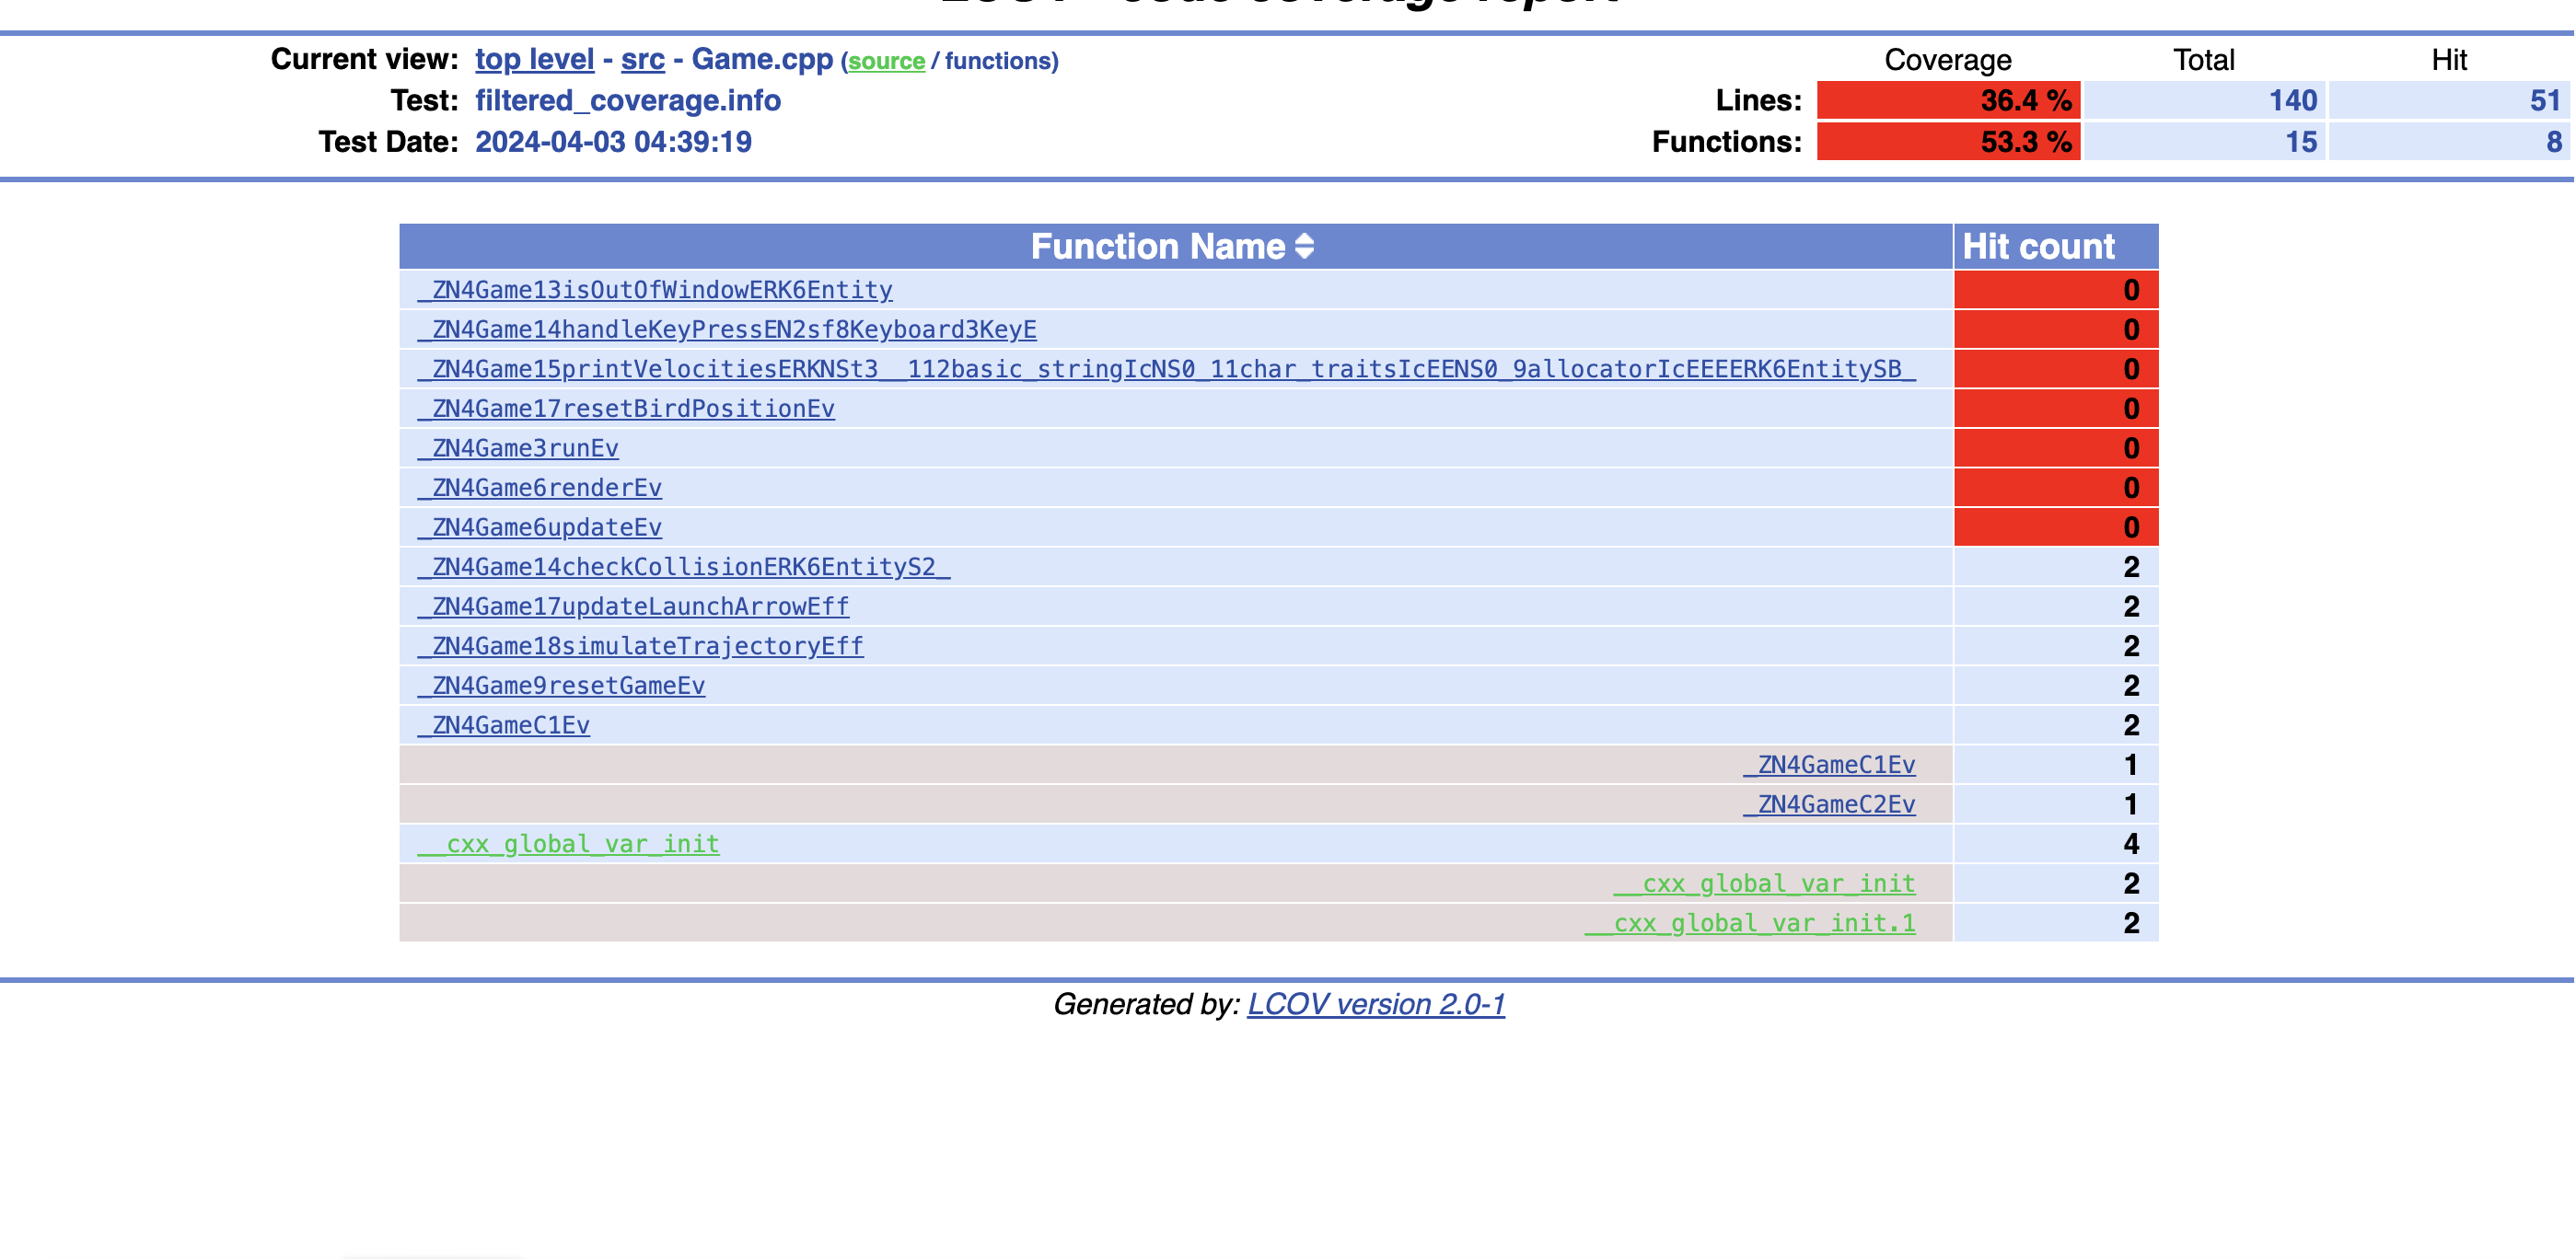
\includegraphics[width=\linewidth]{gamef.png}
    \caption{Test coverage report for Game.cpp, showing another aspect of coverage.}
    \label{fig:game_cpp_other_coverage}
\end{figure}
\FloatBarrier % Prevents figures or tables from floating into the next section

\subsection{Coverage for Specific Test Case}

\begin{figure}[h!]
    \centering
    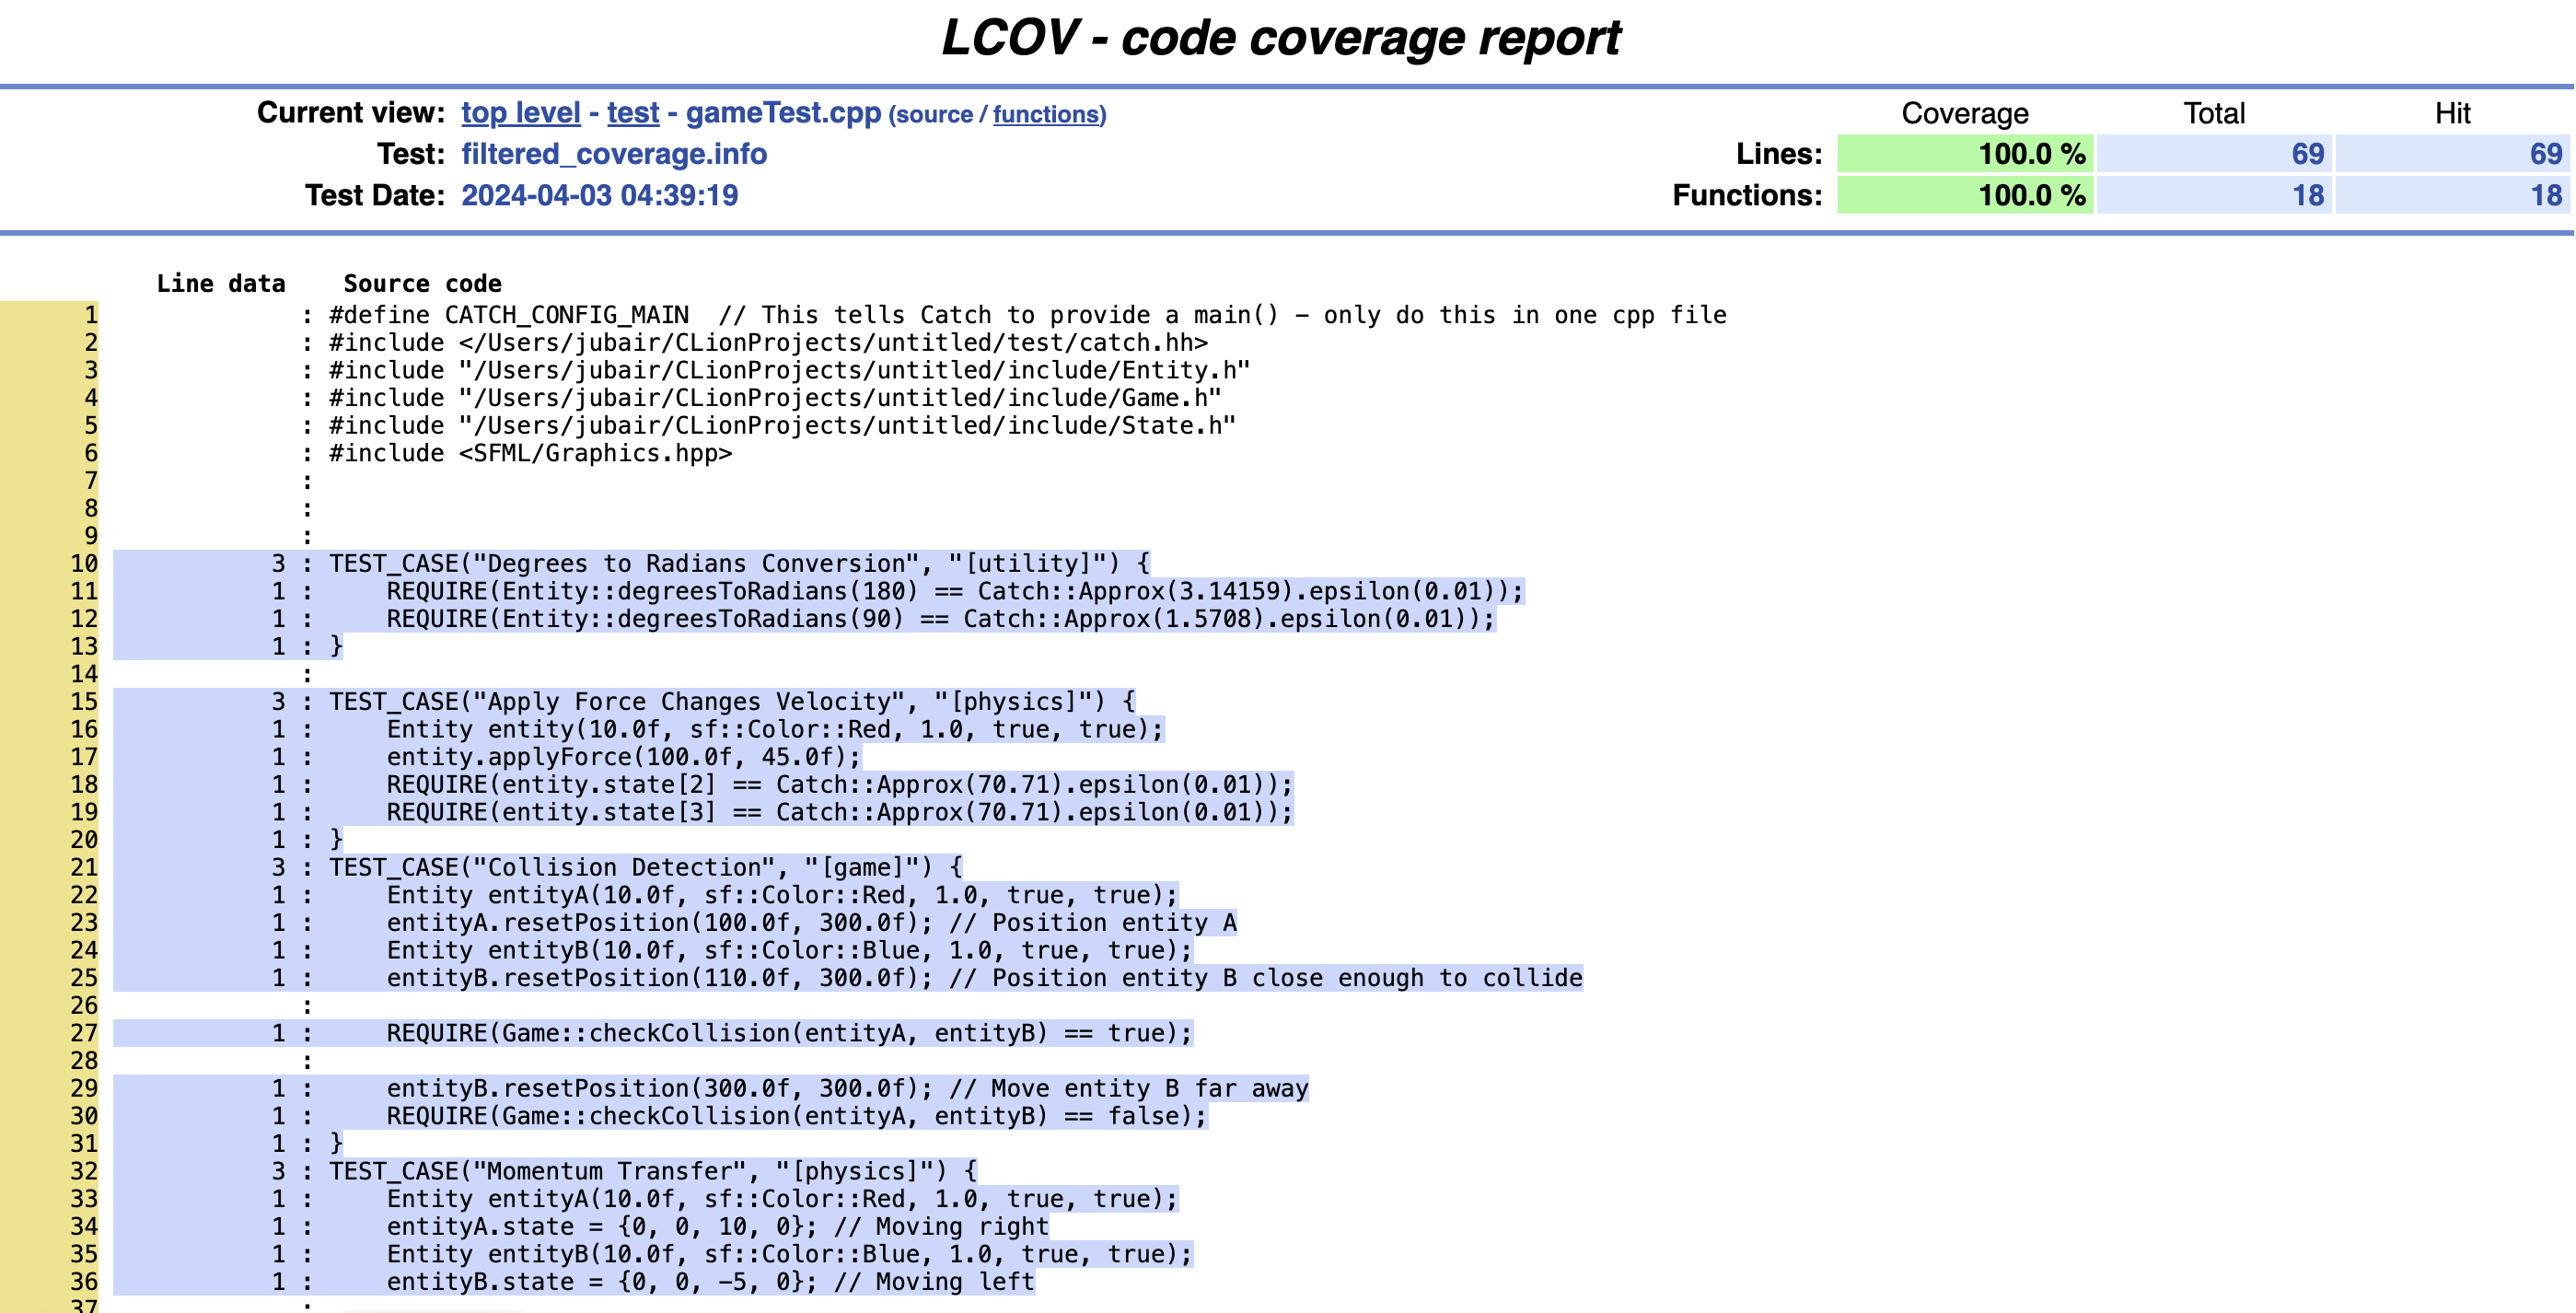
\includegraphics[width=\linewidth]{testcls.png}
    \caption{Test coverage report for a specific test case, showing line coverage.}
    \label{fig:testcase_line_coverage}
\end{figure}

\begin{figure}[h!]
    \centering
    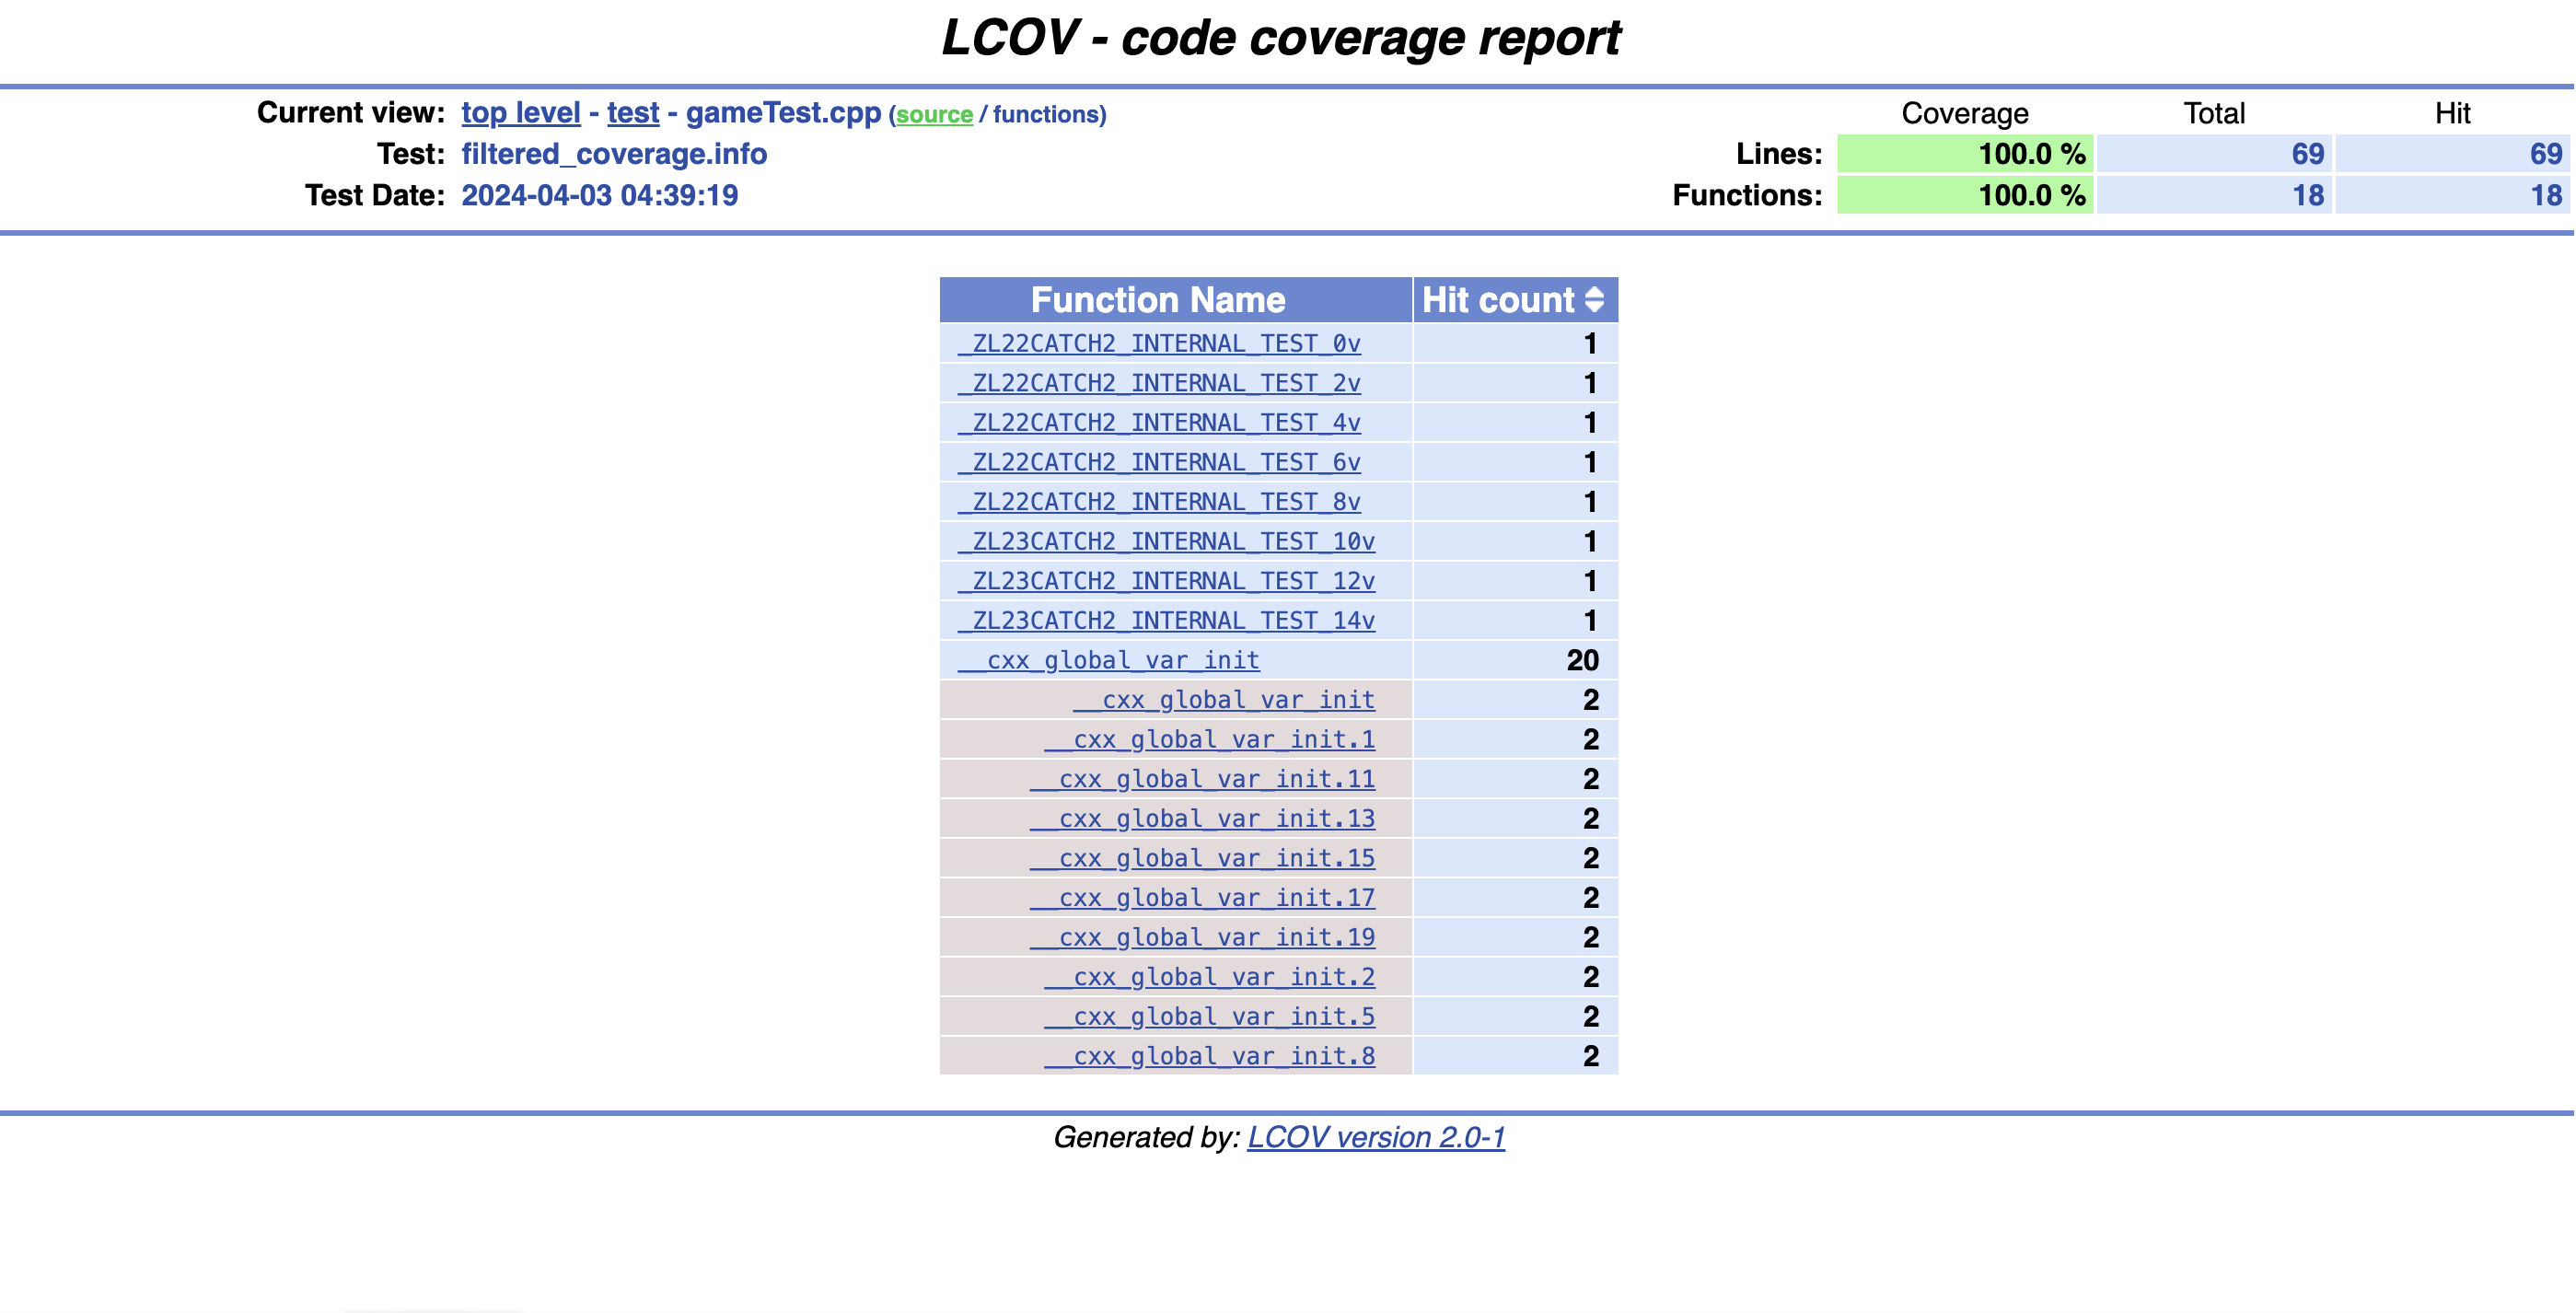
\includegraphics[width=\linewidth]{testc.png}
    \caption{Test coverage report for a specific test case, showing another aspect of coverage.}
    \label{fig:testcase_other_coverage}
\end{figure}
\FloatBarrier % Prevents figures or tables from floating into the next section

\section{Memory Leak Test Results}
\subsection{Leak Test Visualizations}
This section presents the results of memory leak tests performed to ensure the robustness and stability of the application.

\begin{figure}[h!]
    \centering
    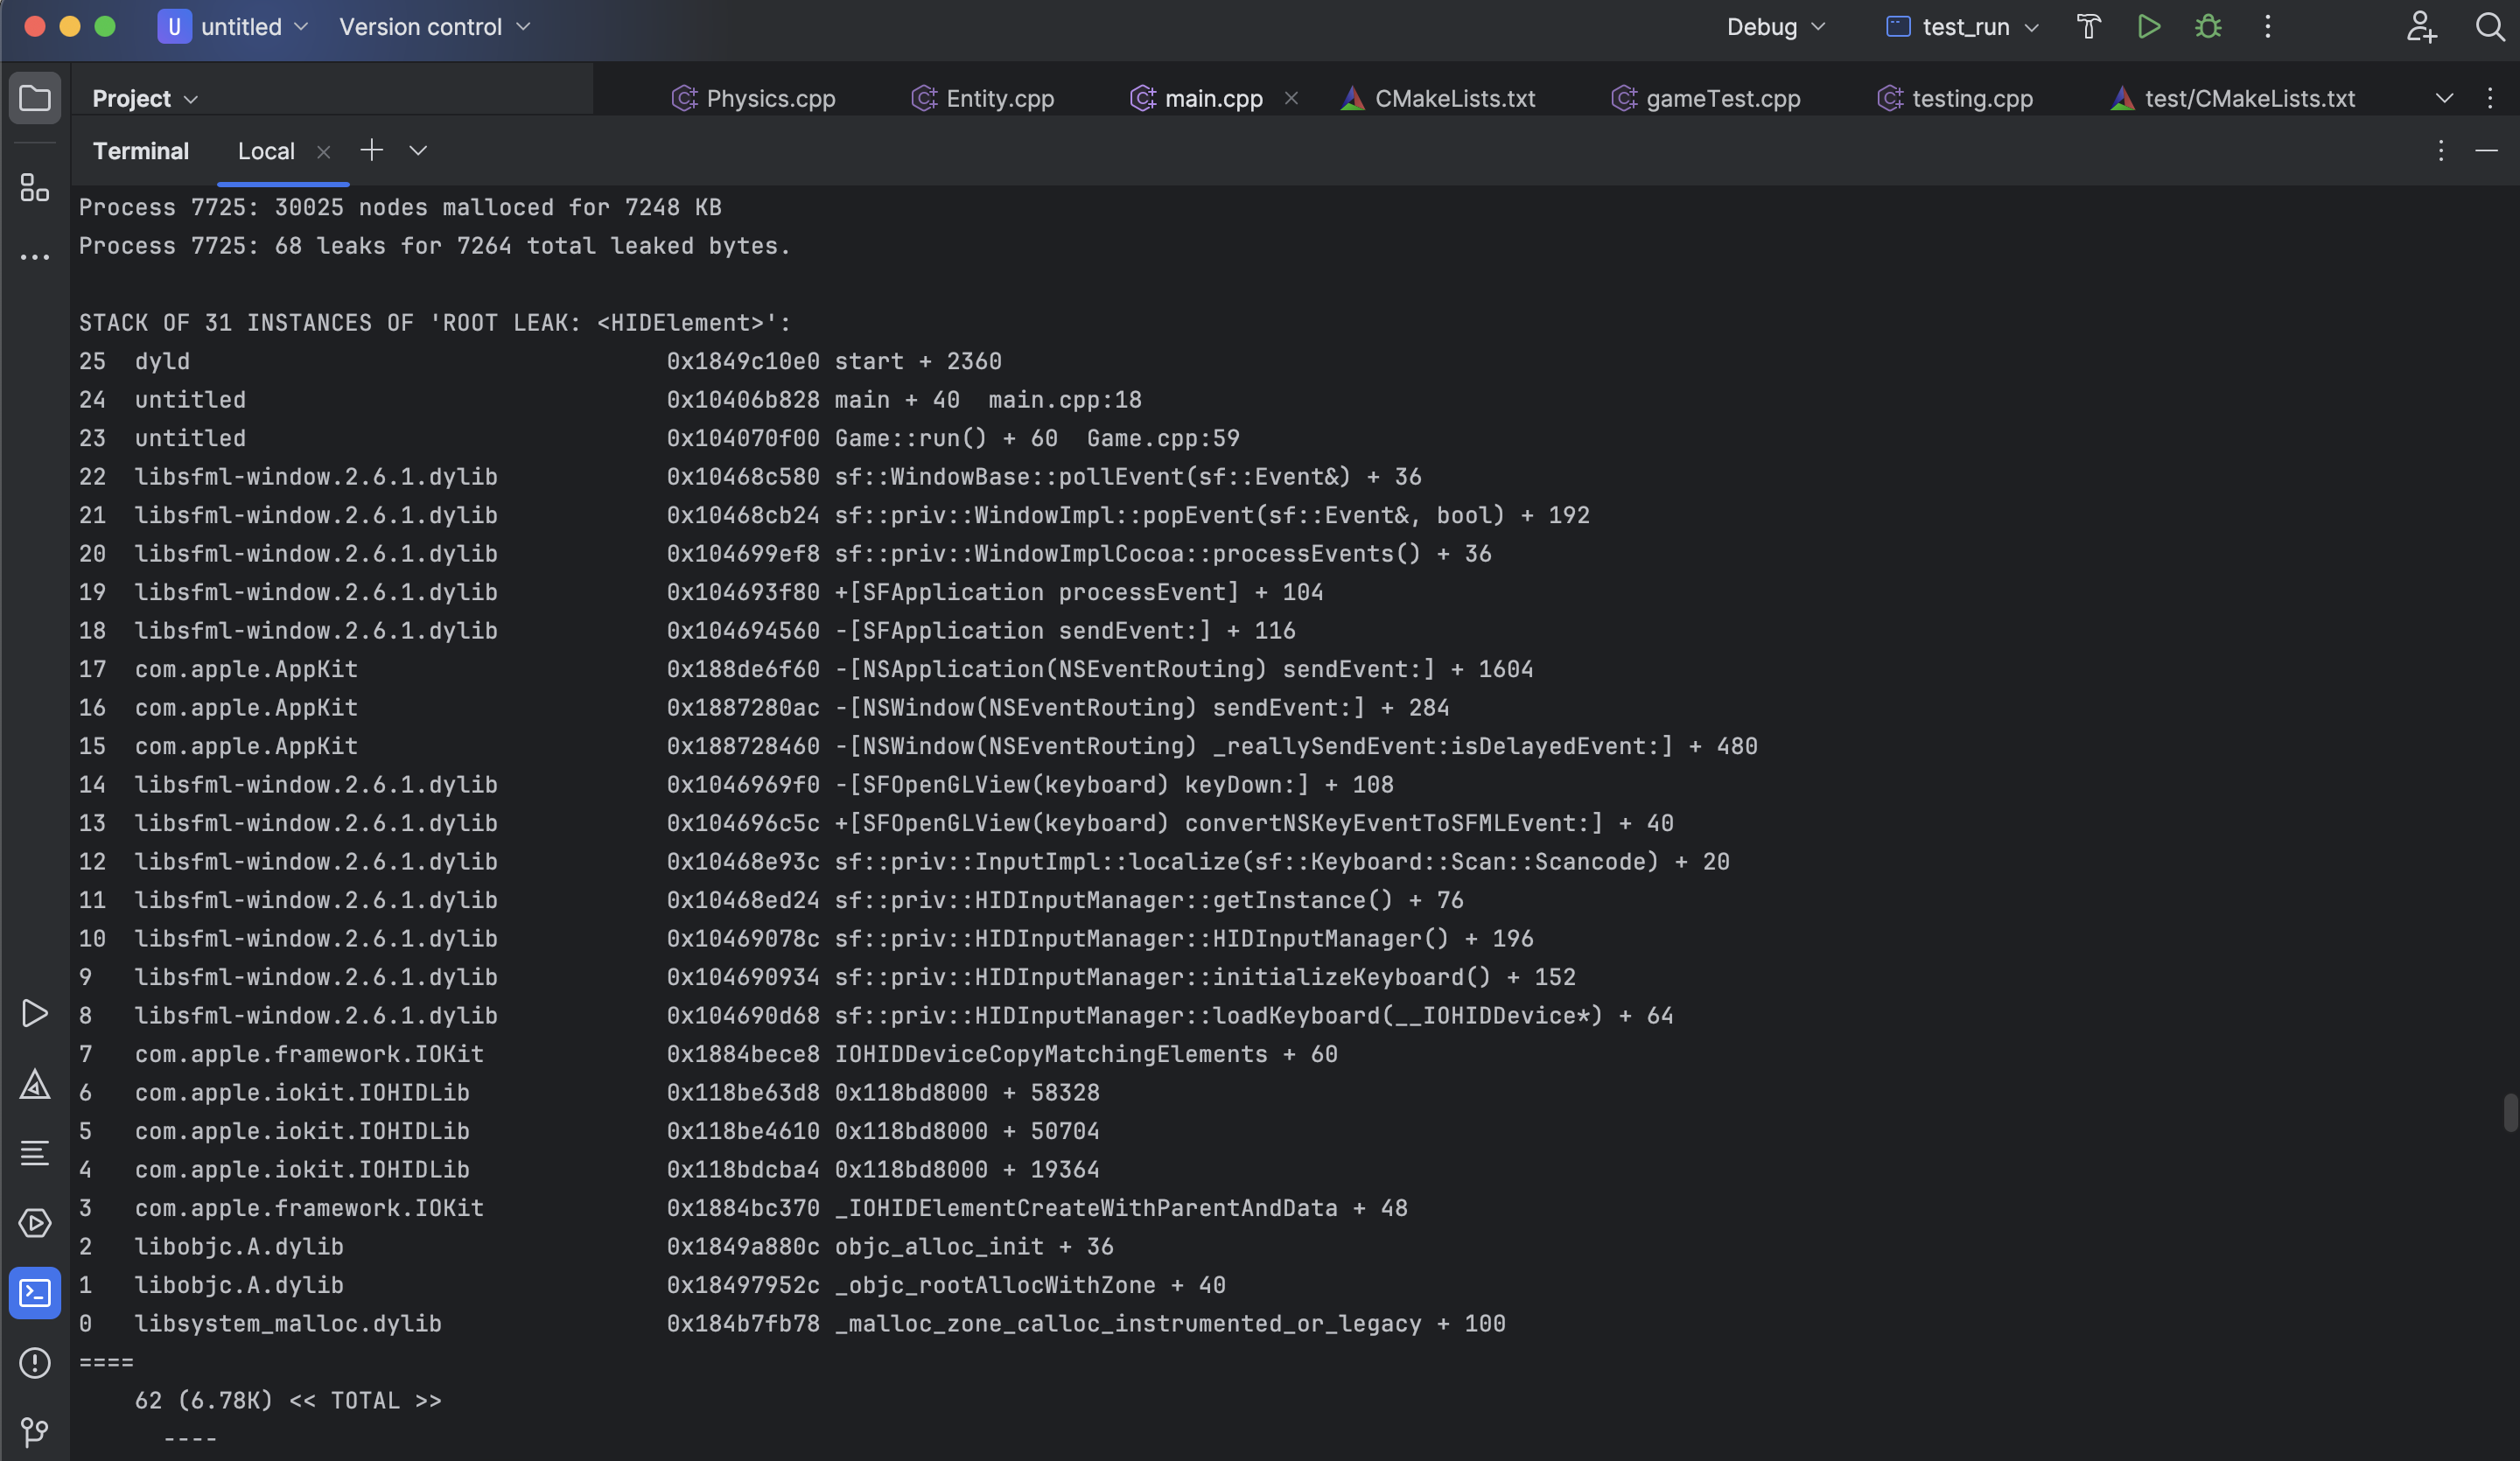
\includegraphics[width=\linewidth]{leaks.png}
    \caption{Memory leak test results showcasing the effective management of memory resources within the application.}
    \label{fig:memory_leak_test}
\end{figure}
\FloatBarrier

\section{Static Code Analysis with Cppcheck}
\subsection{Cppcheck Analysis Results}
Static code analysis was conducted using Cppcheck to identify potential issues in the codebase such as memory leaks, uninitialized variables, and other common coding mistakes.

\begin{figure}[h!]
    \centering
    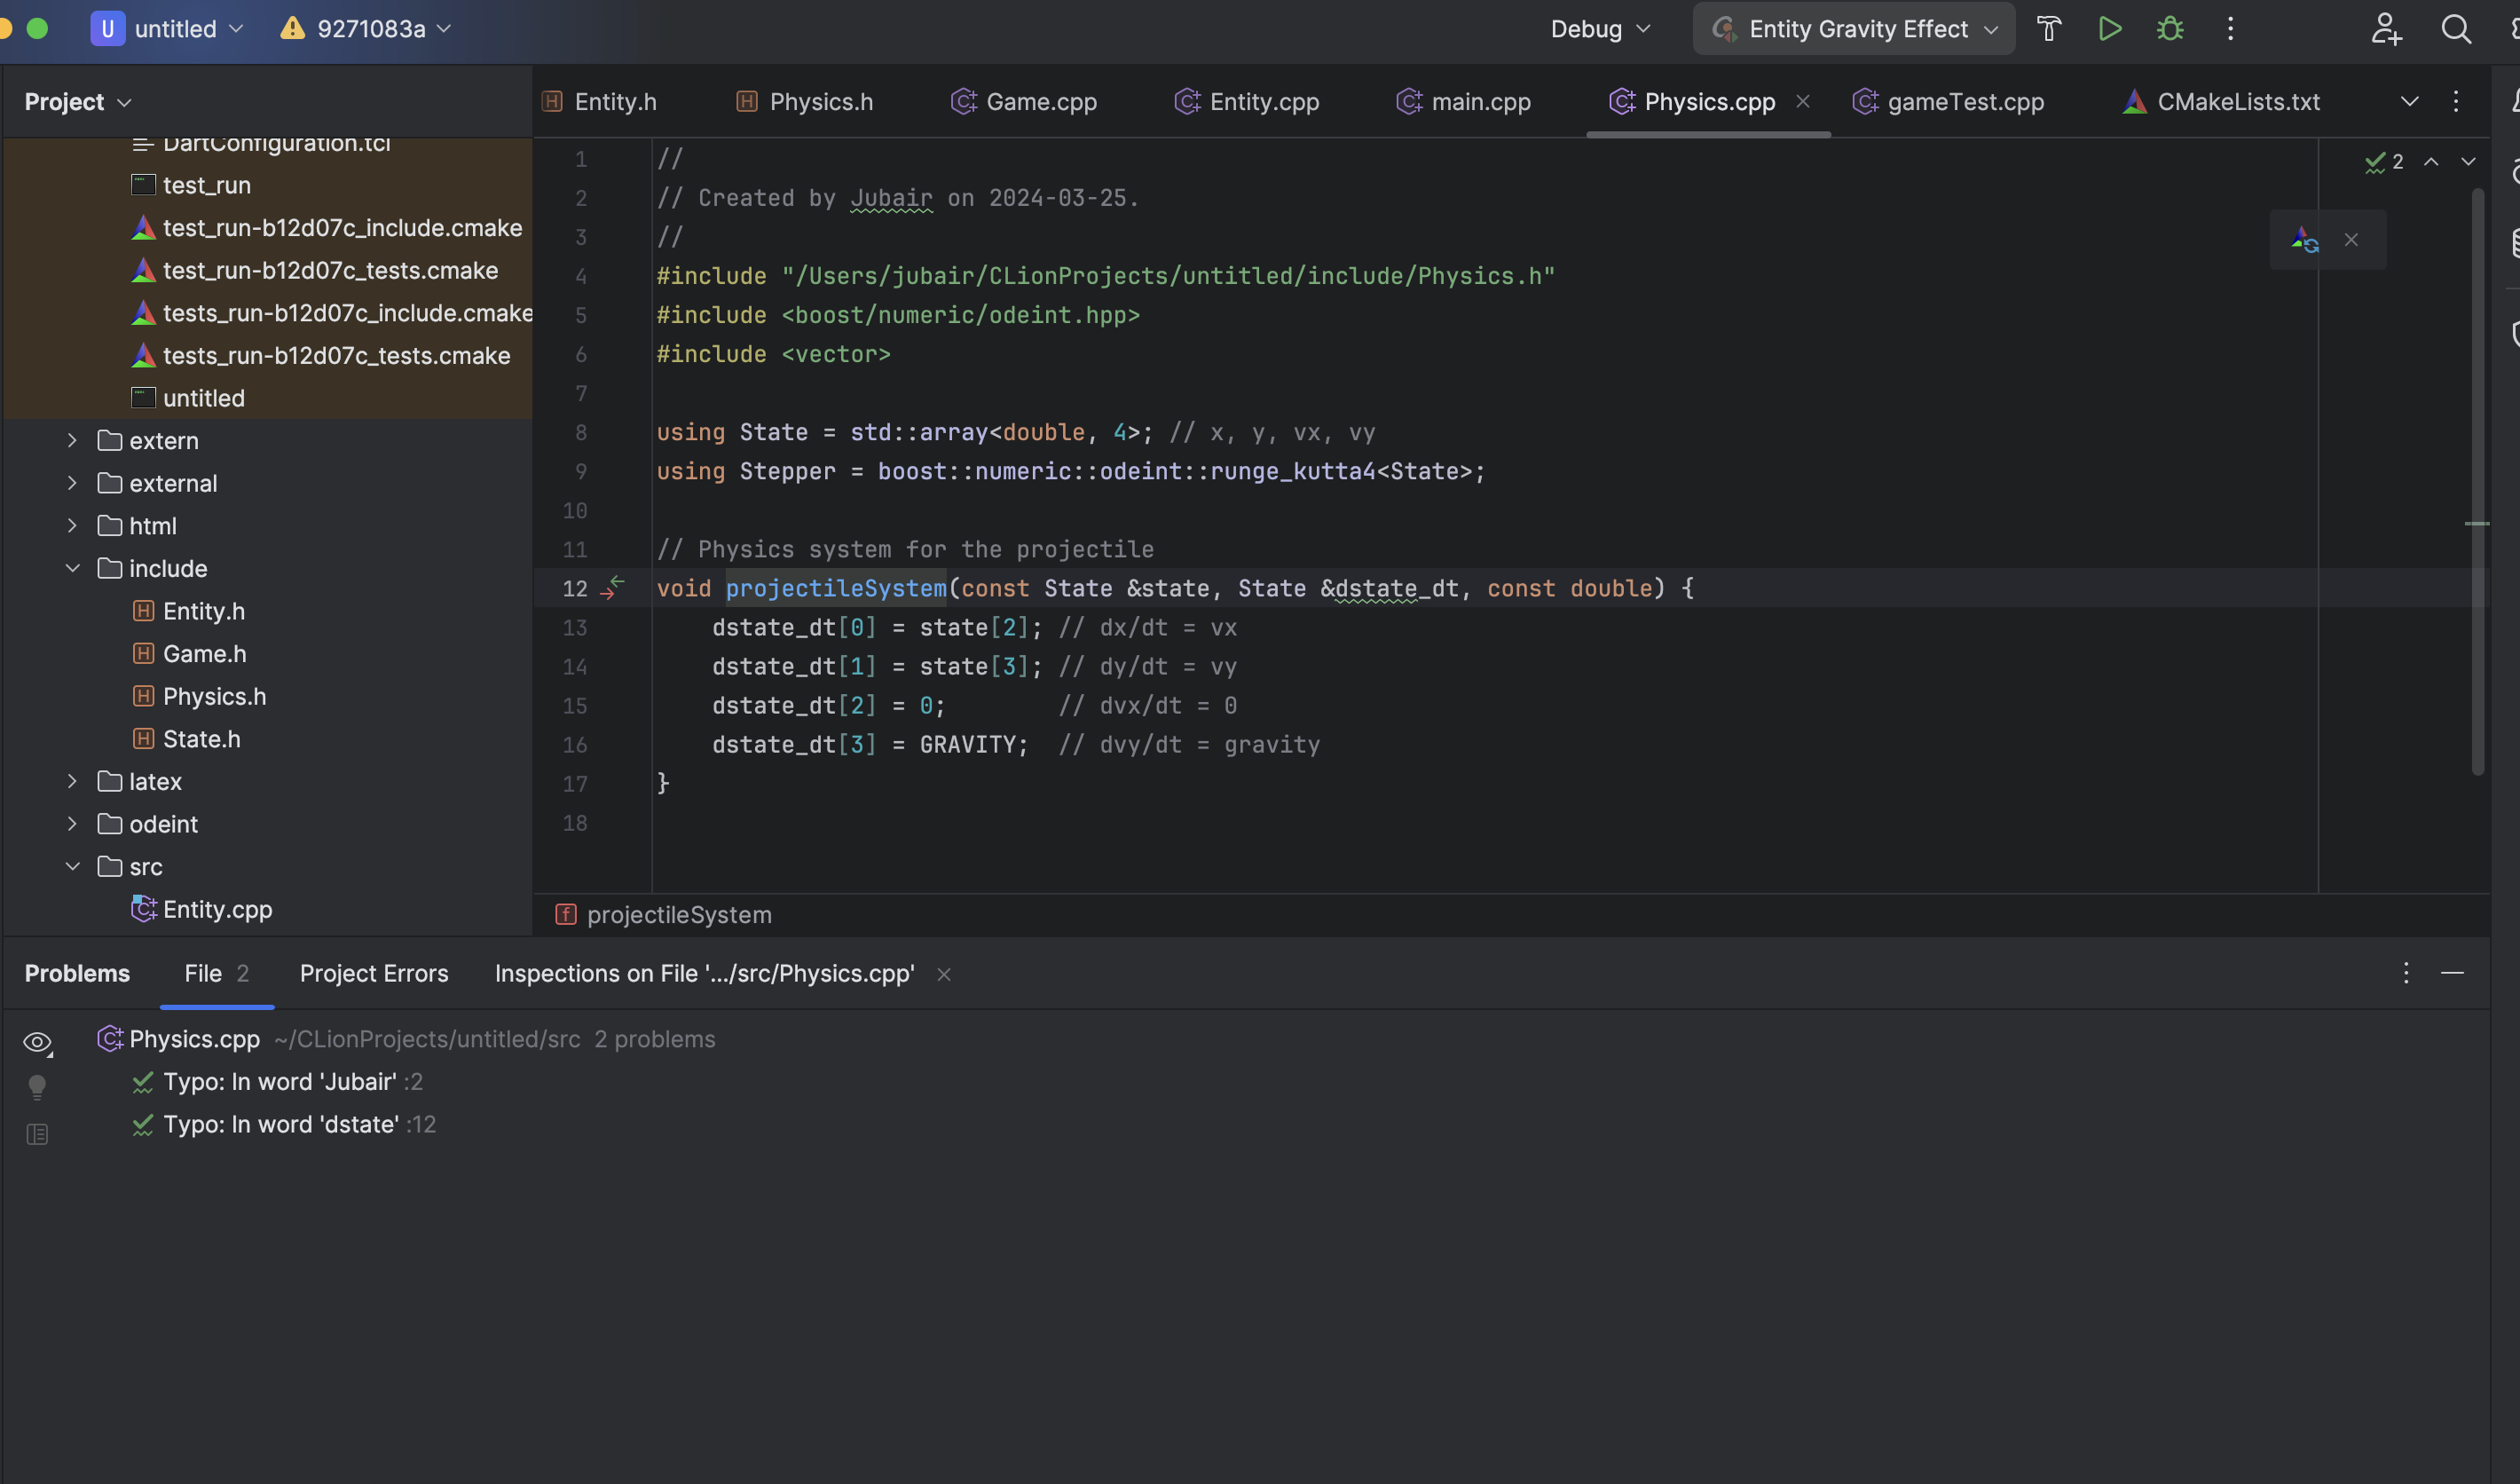
\includegraphics[width=\linewidth]{cpp1.png}
    \caption{Cppcheck analysis results highlighting the areas of the code requiring attention to improve code quality and reliability.}
    \label{fig:cppcheck_results}
\end{figure}
\FloatBarrier

\begin{figure}[h!]
    \centering
    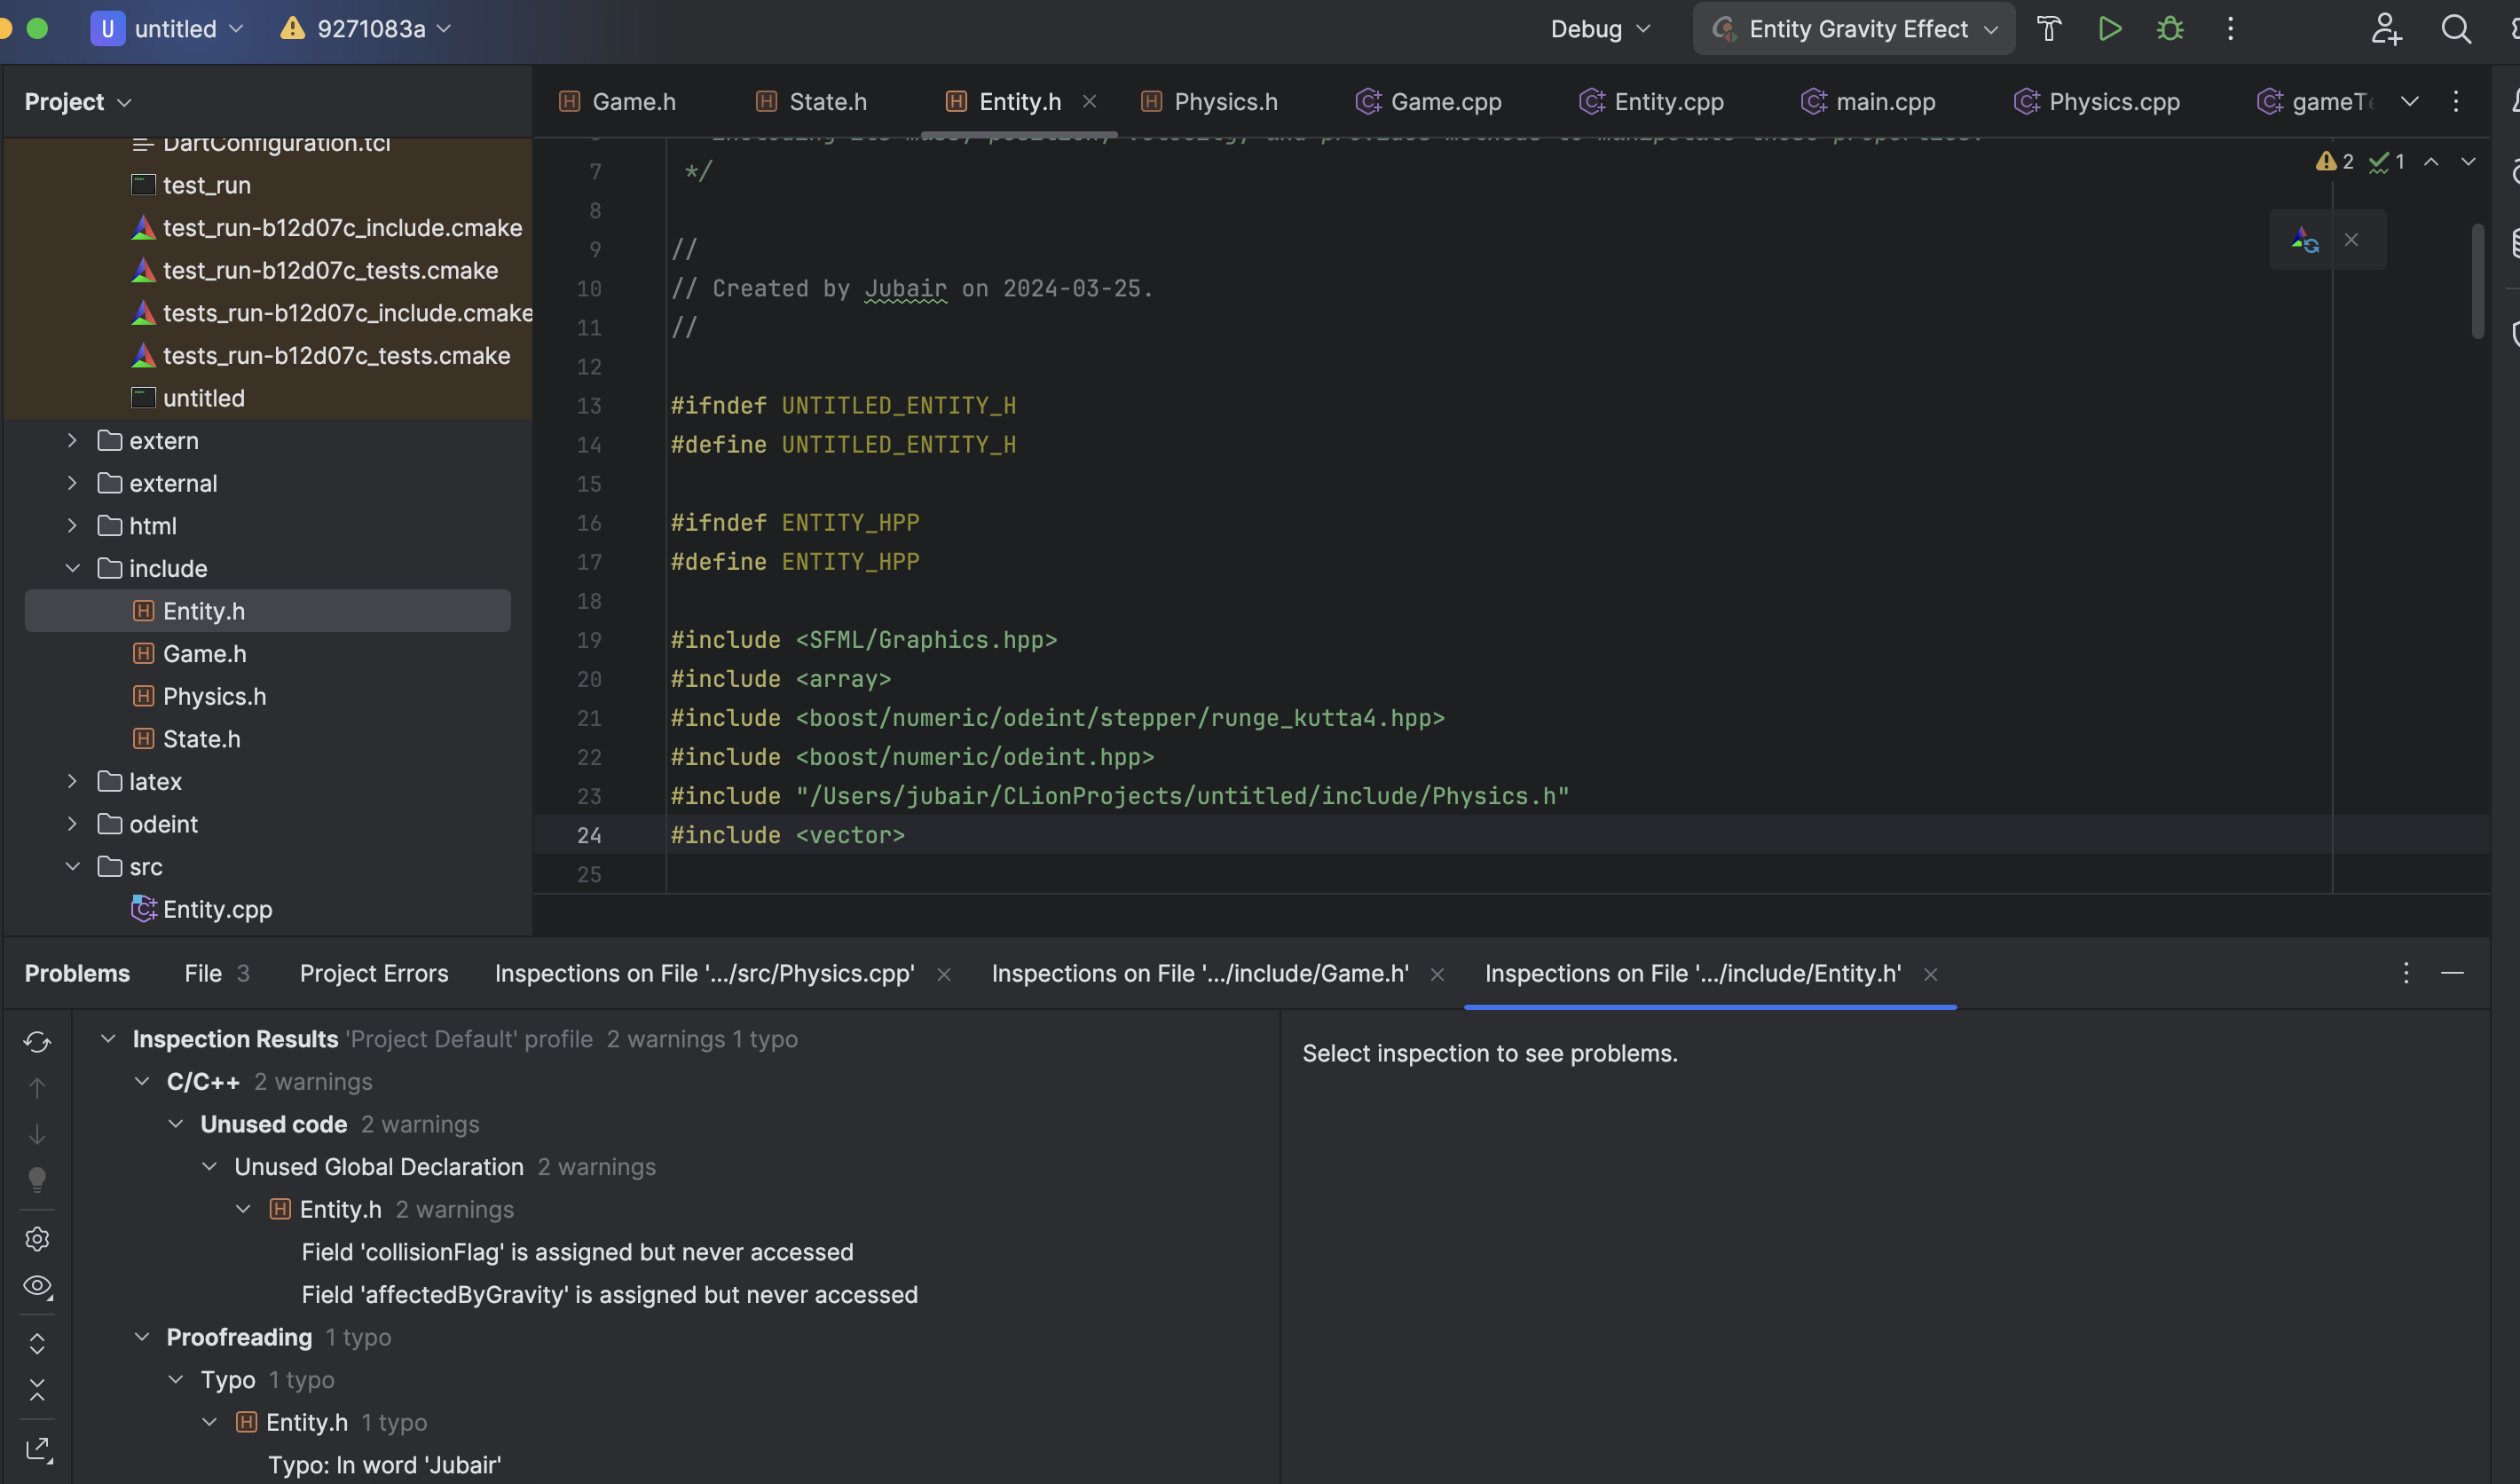
\includegraphics[width=\linewidth]{cpp2.png}
    \caption{Cppcheck analysis results highlighting the areas of the code requiring attention to improve code quality and reliability.}
    \label{fig:cppcheck_results}
\end{figure}
\FloatBarrier

\begin{figure}[h!]
    \centering
    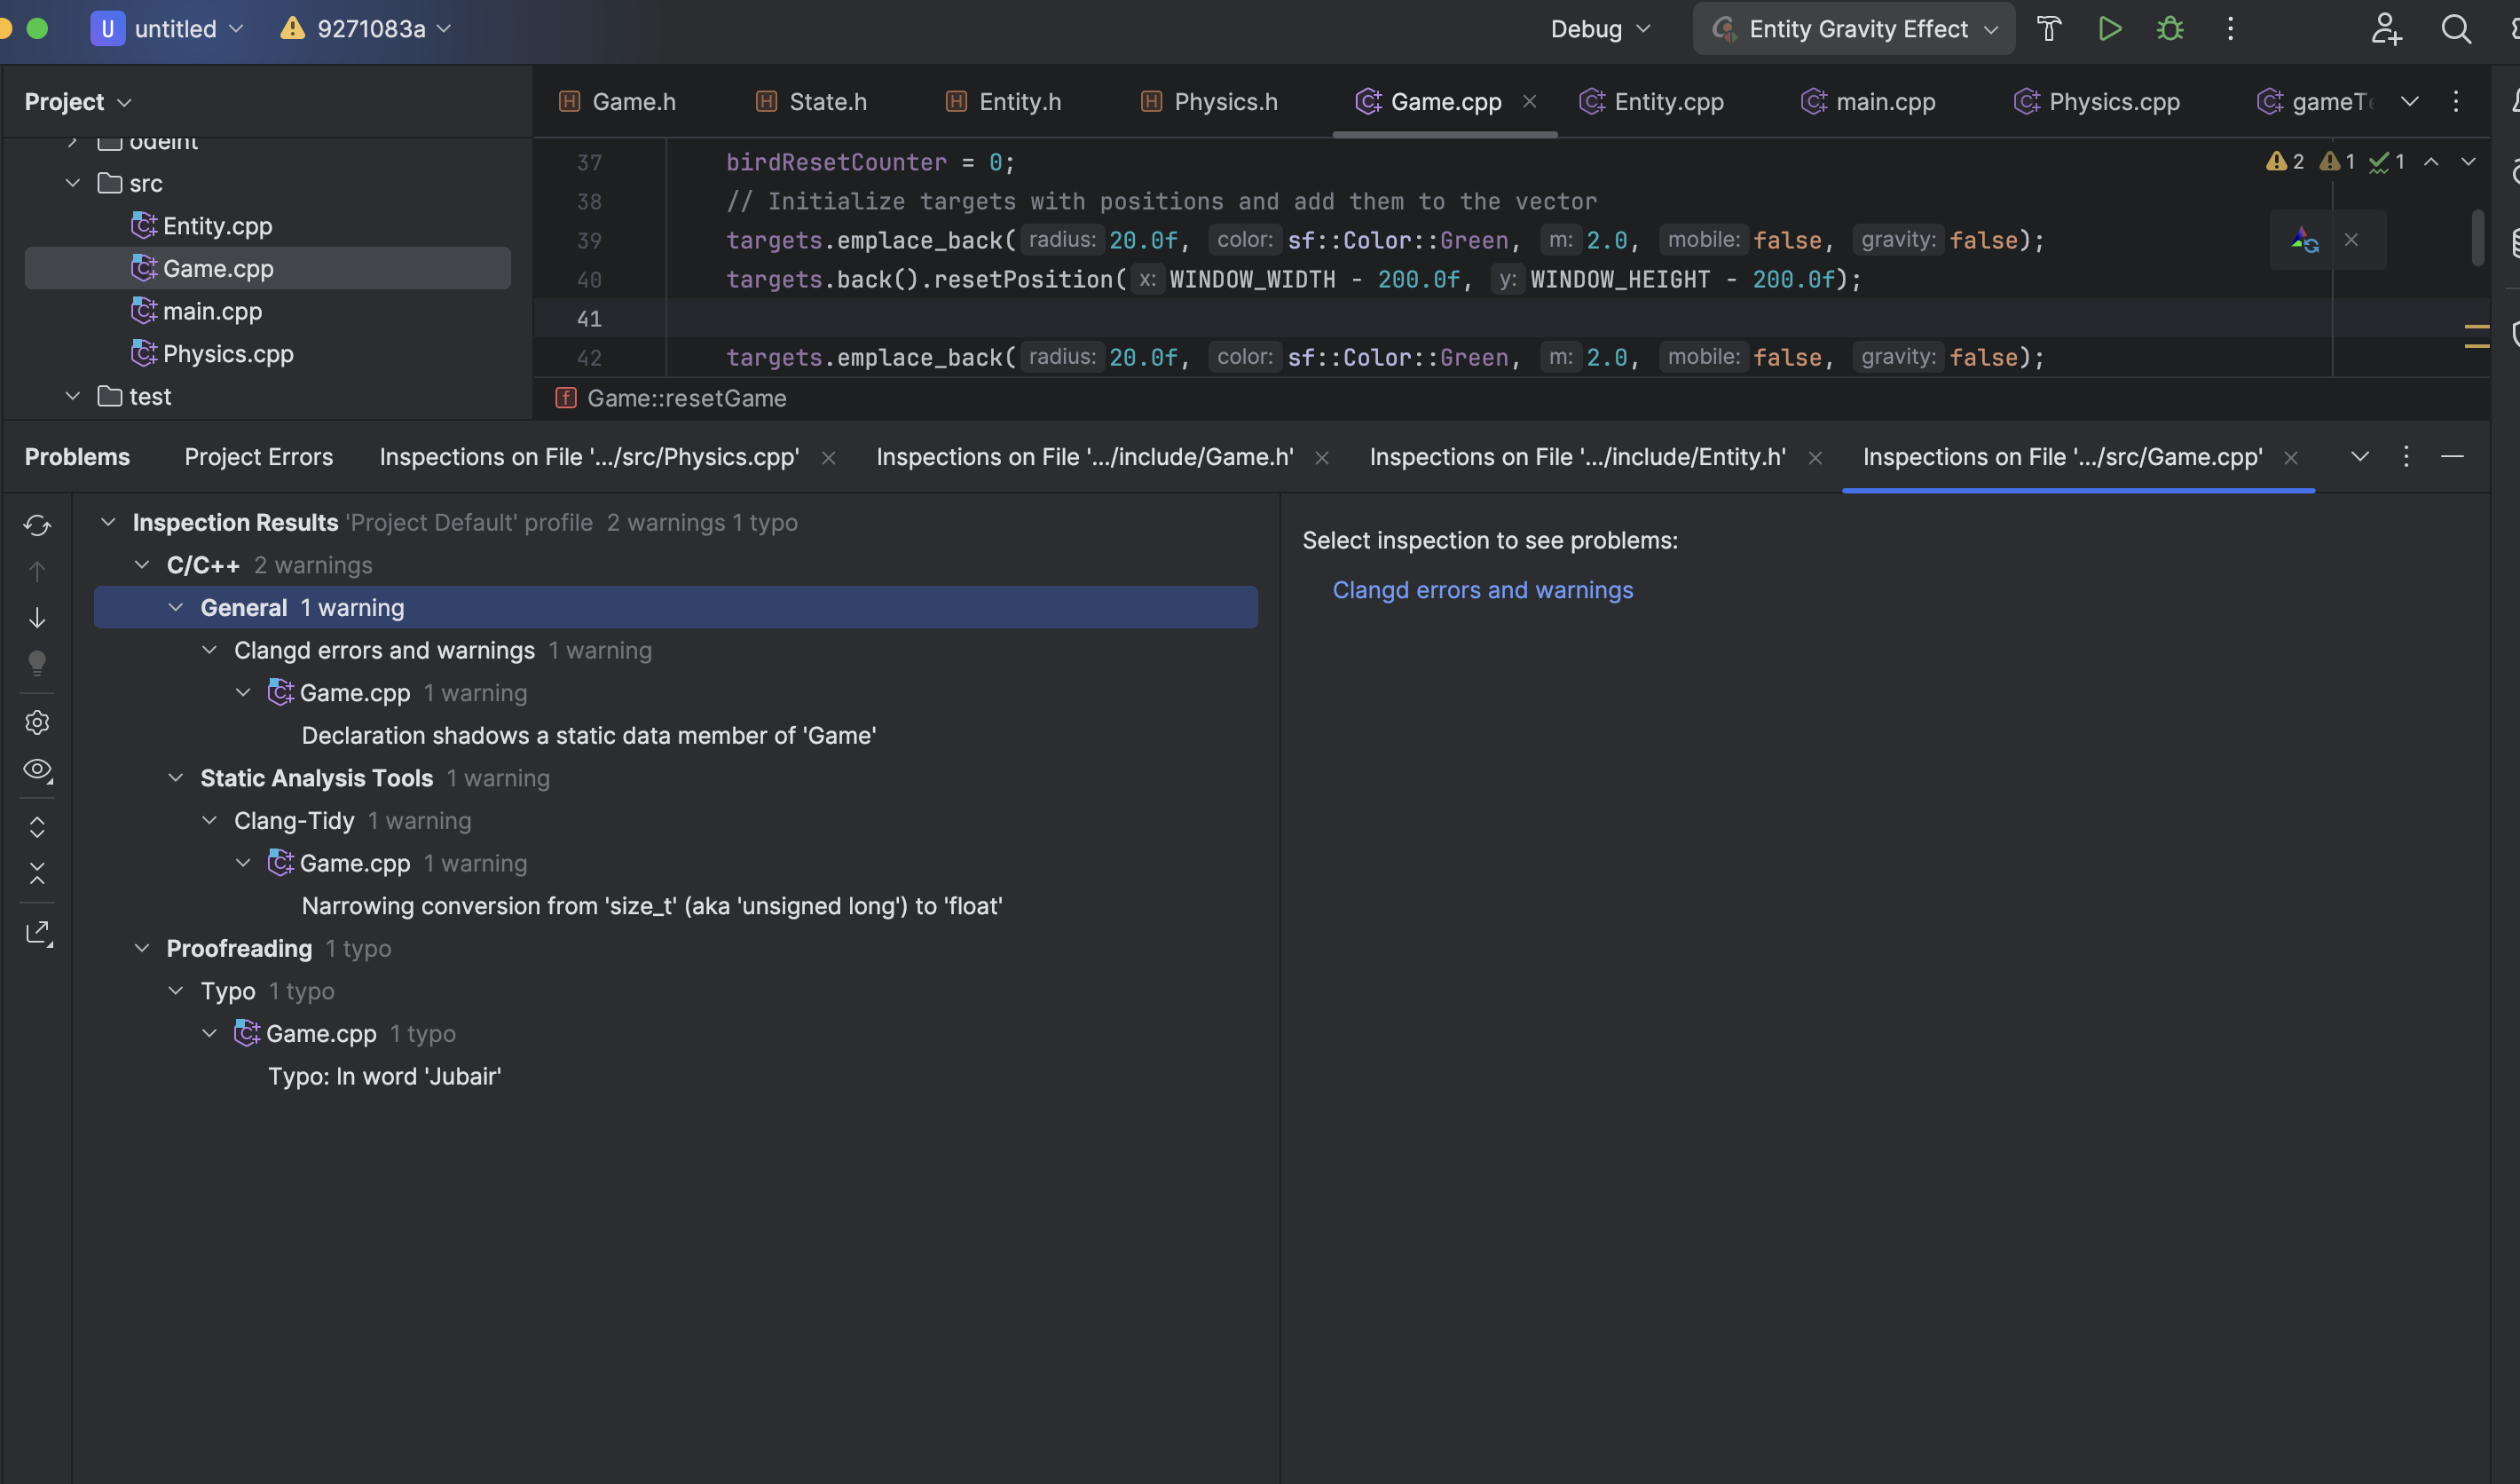
\includegraphics[width=\linewidth]{cpp3.png}
    \caption{Cppcheck analysis results highlighting the areas of the code requiring attention to improve code quality and reliability.}
    \label{fig:cppcheck_results}
\end{figure}
\FloatBarrier

\begin{figure}[h!]
    \centering
    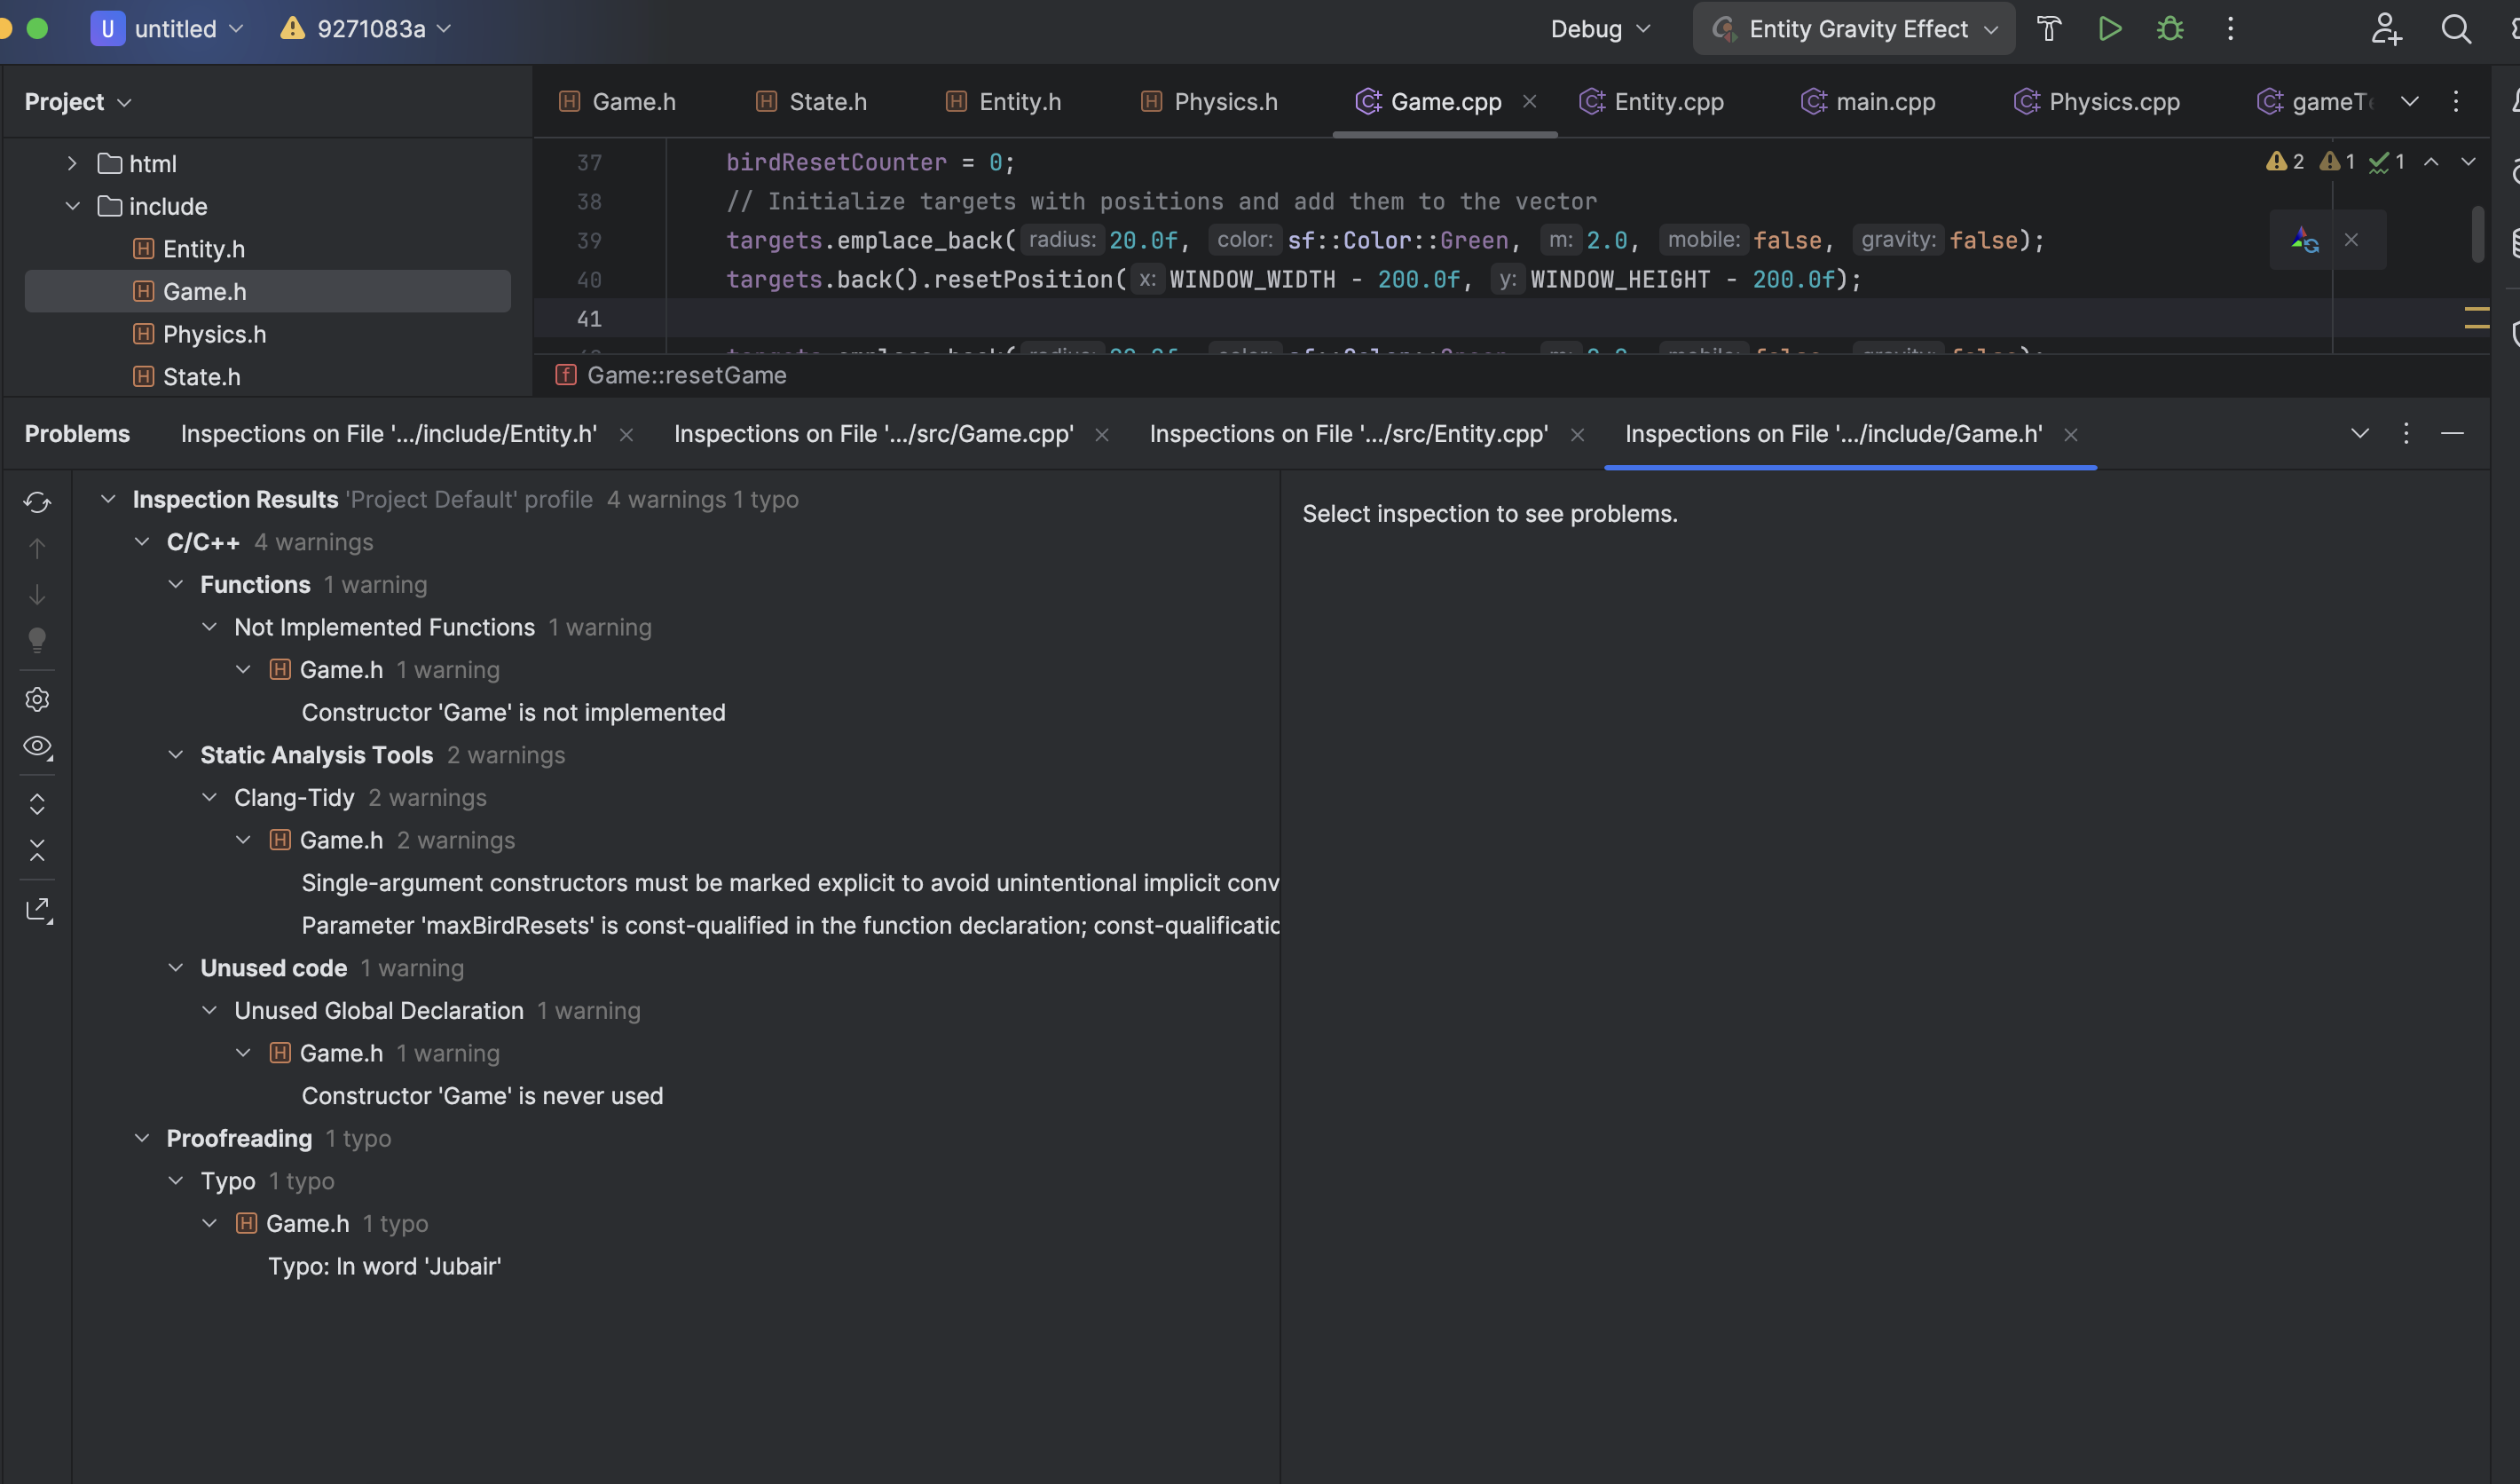
\includegraphics[width=\linewidth]{cpp4.png}
    \caption{Cppcheck analysis results highlighting the areas of the code requiring attention to improve code quality and reliability.}
    \label{fig:cppcheck_results}
\end{figure}
\FloatBarrier

\newpage
\appendix
\section*{Appendix}
\addcontentsline{toc}{section}{Appendix}

\subsection*{A. Reflection on the Verification and Validation Process}
\addcontentsline{toc}{subsection}{A. Reflection on the Verification and Validation Process}
Reflecting on the verification and validation process, it became evident that thorough testing is crucial for identifying and addressing issues early. Despite careful planning, unexpected challenges arose, underscoring the importance of flexibility in our testing approach.

\subsection*{B. Lessons Learned}
\addcontentsline{toc}{subsection}{B. Lessons Learned}
The project highlighted the value of unit testing in maintaining high code quality. It also demonstrated the necessity of comprehensive testing strategies that encompass unit, integration, and system tests.

\subsection*{C. Future Work}
\addcontentsline{toc}{subsection}{C. Future Work}
Future efforts will focus on expanding test coverage, exploring advanced testing frameworks, and continually refining the application based on user feedback and performance metrics.

\subsection*{D. Acknowledgments}
\addcontentsline{toc}{subsection}{D. Acknowledgments}
I extend my graditude to my domain expert, reviewers, Professor, who provided valuable insights and support throughout the project's development.

\subsection*{E. Closing Thoughts}
\addcontentsline{toc}{subsection}{E. Closing Thoughts}
This project has been a journey of learning and growth. I am excited to apply the insights gained to future projects, with a commitment to developing robust, efficient, and user-friendly software.

\end{document}
